% Springer Computer Science Proceedings (splnproc2306) — LaTeX equivalent:
% the official Springer llncs.cls package shipped with the venue template.
\documentclass{llncs}

\usepackage[T1]{fontenc}
\usepackage[utf8]{inputenc}
% Times text+math to match the splnproc2306 Word template's Times New Roman.
\usepackage{newtxtext}
\usepackage{newtxmath}
\usepackage{microtype}
\usepackage{indentfirst} % seragamkan: SEMUA paragraf menjorok, termasuk pertama abis heading
\usepackage{cite}
\usepackage{graphicx}
\usepackage{subcaption}
% LNCS caption style: "Fig. 1." with a period (subcaption/caption would
% otherwise override llncs.cls to "Fig. 1:" — a visible LNCS violation).
\captionsetup{labelsep=period}
\captionsetup[sub]{labelsep=period}
\usepackage{amsmath}
\usepackage{bm}
\usepackage{booktabs}
\usepackage{rotating}
\usepackage{tikz}
\usetikzlibrary{arrows.meta,positioning,fit,backgrounds,calc,shapes.geometric}
\usepackage{xcolor}
\usepackage{fontawesome5}
% Wider text block (Kevin 2026-09-05: "gak peduli template, yang penting
% rapat"): 2.0cm margins on A4 -> 17cm text block, pages fill properly.
\usepackage[a4paper,margin=2cm]{geometry}
% Uniform float-to-text gaps (identical spacing after every figure/table).
\setlength{\textfloatsep}{13pt plus 2pt minus 2pt}
\setlength{\floatsep}{14pt plus 2pt minus 2pt}
\setlength{\intextsep}{14pt plus 2pt minus 2pt}
% Avoid ragged overfull lines around unbreakable \texttt/cite tokens.
\setlength{\emergencystretch}{2.5em}
% Float policy: allow tall figures on top of text pages, and fill float
% pages from the top (LaTeX default pushes them to the bottom).
\renewcommand{\topfraction}{0.95}
\renewcommand{\bottomfraction}{0.6}
\renewcommand{\textfraction}{0.05}
\renewcommand{\floatpagefraction}{0.85}
\makeatletter
\setlength{\@fptop}{4pt}
\setlength{\@fpsep}{10pt plus 1fil}
\setlength{\@fpbot}{0pt plus 1fil}
\makeatother
% Palette for pipeline/architecture diagrams (colorful but professional).
\definecolor{cCapture}{RGB}{33,102,172}
\definecolor{cLandmark}{RGB}{0,136,136}
\definecolor{cNorm}{RGB}{221,132,31}
\definecolor{cModel}{RGB}{178,24,43}
\definecolor{cLogic}{RGB}{94,60,153}
\definecolor{cNet}{RGB}{27,120,55}
\definecolor{cBg}{RGB}{245,245,245}
% --- Manual-figure placeholder: dashed slot to be replaced by a real image ---
% (temporary; see MANUAL_FIGURE_BRIEF.md for the capture/draw spec per figure)
\newcommand{\manualfig}[2]{%
\begin{tikzpicture}
\node[draw=black!50, dashed, line width=1pt, rounded corners=4pt, fill=cBg,
  inner sep=10pt, minimum width=0.94\linewidth, minimum height=35mm,
  align=left, text width=0.84\linewidth] {%
  {\footnotesize\bfseries\color{cModel}[ TEMPORARY PLACEHOLDER --- replace
  with the manual image described in MANUAL-FIGURE-BRIEF.md ]}\\[6pt]
  {\small #1}\\[6pt]
  {\footnotesize\itshape\color{black!60}#2}};
\end{tikzpicture}}
% --- Heading hierarchy (Kevin 2026-09-07): subtle but clear sizes ---
\makeatletter
\renewcommand\section{\@startsection{section}{1}{\z@}%
                      {-18\p@ \@plus -4\p@ \@minus -4\p@}%
                      {12\p@ \@plus 4\p@ \@minus 4\p@}%
                      {\normalfont\Large\bfseries\boldmath
                       \rightskip=\z@ \@plus 8em\pretolerance=10000 }}
\renewcommand\subsection{\@startsection{subsection}{2}{\z@}%
                      {-18\p@ \@plus -4\p@ \@minus -4\p@}%
                      {8\p@ \@plus 4\p@ \@minus 4\p@}%
                      {\normalfont\large\bfseries\boldmath
                       \rightskip=\z@ \@plus 8em\pretolerance=10000 }}
\renewcommand\subsubsection{\@startsection{subsubsection}{3}{\z@}%
                      {-18\p@ \@plus -4\p@ \@minus -4\p@}%
                      {-0.5em \@plus -0.22em \@minus -0.1em}%
                      {\normalfont\normalsize\bfseries\itshape\boldmath}}
\makeatother
\usepackage[hidelinks]{hyperref}
\usepackage{xurl}
\usepackage{enumitem}
\setlist[itemize]{nosep, leftmargin=12pt}
\setlist[enumerate]{nosep, leftmargin=16pt}
% Key-term emphasis: visible but professional (no highlighter).
\newcommand{\kw}[1]{\textbf{#1}}
% Consistent icon set for the pipeline flowchart (FontAwesome 5).
\newcommand{\icam}[1]{\textcolor{#1}{\faVideo}}
\newcommand{\ihand}[1]{\textcolor{#1}{\faHandPaper}}
\newcommand{\ilayers}[1]{\textcolor{#1}{\faLayerGroup}}
\newcommand{\islider}[1]{\textcolor{#1}{\faSlidersH}}
\newcommand{\inet}[1]{\textcolor{#1}{\faBrain}}
\newcommand{\ibars}[1]{\textcolor{#1}{\faChartBar}}
\newcommand{\ikeys}[1]{\textcolor{#1}{\faKeyboard}}
\newcommand{\ivol}[1]{\textcolor{#1}{\faVolumeUp}}
\newcommand{\iwifi}[1]{\textcolor{#1}{\faWifi}}
\newcommand{\iusers}[1]{\textcolor{#1}{\faUsers}}

\title{BISINDO Bridge: Lightweight Dual-Hand Landmark Recognition for
In-Browser Sign Language Communication in Video Meetings}
\titlerunning{BISINDO Bridge: Dual-Hand Landmark Recognition in Video Meetings}

\author{Felicia Gunardi\inst{1}
\and Jouxing Ngo\inst{1}
\and Kevin Pierre Rafael Sabran\inst{1}
\and Muhammad Naufal Dwitama\inst{1}
\and Wiby Aldiputra\inst{1}
\and Gabriel Asael Tarigan\inst{1}}
\authorrunning{F. Gunardi et al.}

\institute{Computer Science Department, BINUS University, Jakarta, Indonesia}

\begin{document}

\maketitle

% ============================================================
\begin{abstract}
Online meetings remain largely inaccessible for millions of
deaf individuals in Indonesia --- mainstream platforms provide little
native support for Bahasa Isyarat Indonesia (BISINDO), and prior BISINDO
recognition research is dominated by heavy sequence models over video that
are rarely deployed as communication tools. We present \kw{BISINDO Bridge},
an end-to-end \kw{dual-hand} recognition system that runs \kw{entirely in
the browser} and integrates into a multi-party video meeting. Each gesture
is encoded as an 84-dimensional vector
($21$ landmarks $\times\,2$ coordinates $\times\,2$ hands) from MediaPipe
Hands, normalized in three stages for position and scale invariance, and
classified by a compact \kw{one-dimensional CNN} (61{,}274 parameters).
On a dual-hand
dataset of 26{,}192 samples (about 1{,}000 per letter; 1{,}192 for
A), the deployed model achieves \kw{98.45\% accuracy} and 98.45\%
weighted F1 on a stratified 15\% hold-out (3{,}929 samples). Converted to
ONNX (241~KB), inference runs on-device via ONNX Runtime Web, so no video
leaves the user's browser. Beyond classification, we implement sentence
composition from gesture delimiters and a \kw{full-mesh WebRTC} meeting
with live letter broadcasting over Google STUN and a best-effort public
TURN fallback; the mesh imposes an $O(n^2)$ connection cost that we
evaluate as a scalability limit. A single-hand ablation reaches 99.12\%
but cannot support the two-handed nature of most BISINDO letters and is
not deployed. We frame the system as a strong, honestly-evaluated
\kw{proof-of-concept} rather than a production-ready deployment.
\end{abstract}

\keywords{BISINDO (Indonesian Sign Language) \and Dual-Hand Gesture
Recognition \and MediaPipe \and 1D-CNN \and ONNX Browser Inference
\and WebRTC}


% ============================================================
\section{Introduction}

Communication underpins participation in education, work, and social
life. For people with hearing and speech impairments in Indonesia, Bahasa
Isyarat Indonesia (BISINDO) is a primary language, yet unfamiliar to most
hearing people. Virtual meeting tools such as Google Meet and Zoom
amplify this gap: they center spoken language and text chat, leaving deaf
participants dependent on scarce human interpreters.

Two sign systems coexist in Indonesia. SIBI is the formally standardized
system designed for consistency in instruction; BISINDO is the natural
sign language that Deaf communities actually use in daily conversation,
regional and continuously evolving. Crucially for recognition, the
BISINDO manual alphabet is signed predominantly with \emph{both} hands
(only a few letters reduce to one), so any practical recognizer for the
language people actually sign must accept two-hand input --- not as an
option, but as a requirement. Meeting platforms offer neither
interpreters at scale nor any keypoint-based signing support, making the
accessibility gap structural rather than cosmetic.

Computer vision can reduce that barrier. MediaPipe
Hands~\cite{mediapipehands2020} estimates 21 anatomical landmarks per
hand on-device, enabling recognition from sparse keypoints rather than
raw pixels. For BISINDO, prior work mostly uses sequence models
(LSTM, CNN-LSTM) over video~\cite{auziqni2022,bisindo-lstm-2023,cnn-lstm-bp},
which reach competitive offline accuracy but are heavy for browser
deployment and seldom close the loop into a usable meeting product.
Lightweight \emph{single-frame} dual-hand classification, deployed as an
accessible communication tool, remains underexplored.

This paper presents \kw{BISINDO Bridge}, combining dual-hand landmark
extraction, a compact 1D convolutional classifier, browser-based ONNX
inference, and a WebRTC meeting with sentence building and live
broadcasting (Fig.~\ref{fig:system}). Our contributions:
\begin{itemize}
\item a \kw{dual-hand landmark pipeline}: $21 \times 2 \times 2 = 84$
features per frame with three-stage normalization;
\item a \kw{lightweight 1D-CNN} (61{,}274 parameters) trained on
26{,}192 samples, reaching \textbf{98.45\%} accuracy and weighted F1 on
3{,}929 held-out samples, independently re-evaluated;
\item \kw{privacy-preserving browser deployment}: PyTorch$\to$ONNX
(241~KB) with numerical parity better than $4\times10^{-6}$ and no
server-side vision;
\item an \kw{end-to-end meeting product} (full-mesh WebRTC, sentence
builder with hold gestures, TTS) with ICE-restart recovery, plus an
honest evaluation of full-mesh scalability.
\end{itemize}

The remainder of this paper is organized as follows.
Section~\ref{sec:related} positions the work against prior BISINDO
recognizers. Section~\ref{sec:overview} outlines the system and its
design goals, and Section~\ref{sec:methodology} details the dataset,
normalization, and classifier. Section~\ref{sec:impl} covers the
browser-side implementation, Section~\ref{sec:experiments} reports
results, Section~\ref{sec:limitation} discusses limitations, and
Section~\ref{sec:conclusion} concludes.


% ============================================================
\section{Related Work}
\label{sec:related}

\subsection{Sign Language Recognition}
Sign language recognition has moved through three input regimes. Early
systems classify RGB frames directly with 2D CNNs; they reach high
accuracy but inherit the full image as input, which makes them sensitive
to background and lighting and expensive at the
edge~\cite{deep-survey,deepsign-access,hand-review}. Skeleton-based
methods replace pixels with tracked joint coordinates, cutting input
dimensionality by orders of magnitude while keeping the pose structure
that defines a sign; reviews of the field treat this representation as a
standard route to real-time recognition~\cite{deep-survey,hand-review}.
A third regime applies sequence models (LSTM, CNN--LSTM) over landmark
or frame streams to capture temporal dynamics, at the cost of larger
models and higher latency.

For BISINDO specifically, published systems cluster in the second and
third regimes. Auziqni~\cite{auziqni2022} combines MediaPipe Holistic
with an LSTM and reports about 97\% on 780 recorded sequences;
evaluation is offline, on video clips rather than live input. Afwan et
al.~\cite{bisindo-lstm-2023} classify skeletal features with an LSTM
and report roughly 93\% validation accuracy on alphabetic gestures.
Aljabar and Suharjito~\cite{cnn-lstm-bp} stack a CNN--LSTM hybrid over
video. Fadzli and Rahardi~\cite{bisindo-cnn-mediapipe} compare
MobileNetV3 and EfficientNetV2B0 on MediaPipe landmark input with a
mobile target. Three
gaps separate them from a usable communication tool: accuracy is
measured offline on pre-recorded input, the models target phones or
standalone scripts rather than a browser, and none places recognition
inside a live meeting where several people read the letters. This work
differs on all three counts.

\subsection{Hand Landmark Extraction}
MediaPipe Hands~\cite{mediapipehands2020,mediapipe-framework} detects
up to two hands and returns 21 landmarks per hand (the wrist plus four
joints on each finger), estimated on-device in real time on CPU. A raw
frame at 640$\times$480 carries roughly $9.2\times10^{5}$ pixel
values; the landmark representation reduces the information relevant to
hand pose to 42 or 84 numbers --- about four orders of magnitude. The
layout also mirrors how fingerspelling is articulated: each finger
contributes one joint chain rooted at the shared wrist, so letter
contrasts --- a curled index versus an extended one, fingertips touching
versus apart --- appear directly as differences between adjacent
landmark positions rather than as global image shifts. The
sparse form is also robust to cluttered backgrounds and lighting shifts,
and it lets the whole pipeline run inside a browser tab without pixels
leaving the device. The trade-off is dependence on tracker quality: when
the tracker misses a hand, the classifier sees an all-zero block, which
our normalization leaves unchanged (Section~\ref{sec:norm}).

\subsection{One-Dimensional CNNs for Gestures}
A 1D convolution slides over an ordered numerical sequence --- sensor
streams, audio, or a flattened landmark vector --- and learns local
patterns with far fewer parameters than an image CNN needs. Al Mudawi et
al.~\cite{1d-cnn-healthcare} apply the idea to daily-life hand gestures
from low-dimensional signals; Kumar et al.~\cite{mediapipe-review}
combine MediaPipe output with CNN classifiers for real-time ASL. For
landmark input the fit is structural: neighbouring positions in the
vector are neighbouring joints, so a width-3 kernel covers each joint
together with its immediate neighbours, without inventing the 2D spatial
grid that flattened coordinates do not have. Stacking such kernels
deepens the effective receptive field: a third layer sees each joint in
the context of its neighbours' neighbours, enough to capture the overall
hand shape without ever forming an image. Because the alphabet task here
is single-frame --- every letter is a static posture --- no recurrent
memory is needed, so the classifier stays minimal and per-frame latency
stays low. The resulting models are
small enough to run where this paper needs them, inside the browser.

\subsection{Research Gap}
Two gaps motivate this work. First, BISINDO classification that runs
in-browser on static frames is less studied than video-sequence models:
the systems above assume recorded clips and none reports a browser-only
deployment. Second, published work generally stops at accuracy tables. A
fingerspelling aid is only useful inside the place where deaf
participants actually communicate --- the meeting itself --- which
requires combining recognition with sentence building, edit gestures,
and multi-party video. We address both gaps with a deployed dual-hand
1D-CNN and a WebRTC collaboration stack, and we report the failure modes
of the full system rather than classifier accuracy alone
(Section~\ref{sec:syseval}).
Figure~\ref{fig:gap} places this work against the systems above on the
three axes where they diverge.

\begin{figure}[t]
\centering
\resizebox{0.85\textwidth}{!}{%
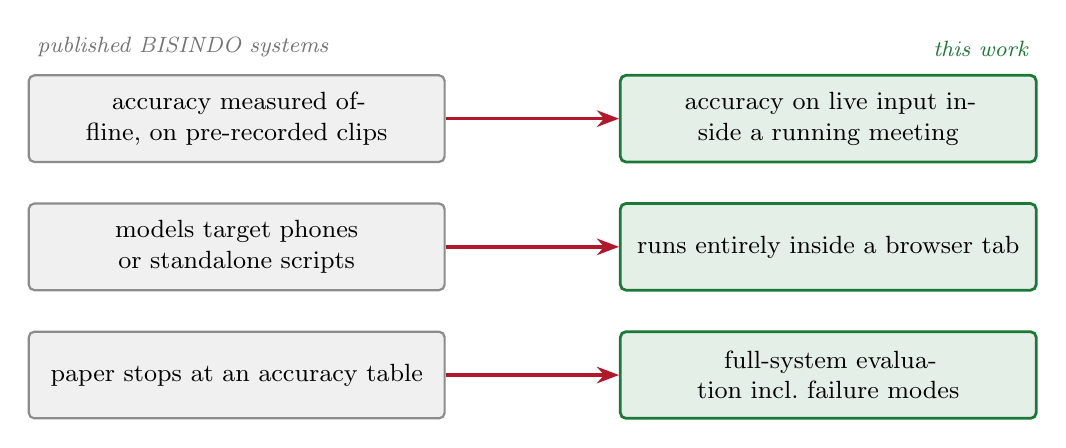
\begin{tikzpicture}[
  font=\small,
  prior/.style={rectangle, rounded corners=2pt, draw=black!45, line width=0.8pt,
    fill=black!6, align=center, inner sep=4pt, minimum height=11mm, text width=50mm},
  ours/.style={rectangle, rounded corners=2pt, draw=cNet, line width=1pt,
    fill=cNet!12, align=center, inner sep=4pt, minimum height=11mm, text width=50mm},
  gapar/.style={-{Stealth[length=2.8mm]}, line width=1.2pt, draw=cModel},
]
\node[prior] (p1) {accuracy measured offline, on pre-recorded clips};
\node[ours, right=22mm of p1] (o1) {accuracy on live input inside a running meeting};
\node[prior, below=5mm of p1] (p2) {models target phones or standalone scripts};
\node[ours, right=22mm of p2] (o2) {runs entirely inside a browser tab};
\node[prior, below=5mm of p2] (p3) {paper stops at an accuracy table};
\node[ours, right=22mm of p3] (o3) {full-system evaluation incl.\ failure modes};
\draw[gapar] (p1) -- (o1);
\draw[gapar] (p2) -- (o2);
\draw[gapar] (p3) -- (o3);
\node[font=\footnotesize\itshape, text=black!55, anchor=south west]
  at ([yshift=1mm]p1.north west) {published BISINDO systems};
\node[font=\footnotesize\itshape, text=cNet, anchor=south east]
  at ([yshift=1mm]o1.north east) {this work};
\end{tikzpicture}}
\caption{Three gaps between published BISINDO recognition systems and a
usable communication tool, and where
\kw{BISINDO Bridge} sits on each.}
\label{fig:gap}
\end{figure}

In short, the missing piece is not another recognizer but the bridge
from one: a classifier small enough to run in every participant's
browser, paired with the meeting plumbing that turns recognized letters
into participation --- speech output, shared text, and sessions that
survive network hiccups.


% ============================================================
\section{System Overview}
\label{sec:overview}

\begin{figure}[t]
\centering
\manualfig{Ten-stage end-to-end pipeline drawn as two serpentine rows joined by a wrap-around connector, enclosed in a dotted on-device boundary.}{Row 1 (left to right): Webcam frame -> MediaPipe Hands (2 x 21 landmarks) -> Flatten (84) -> Normalize (3 stages) -> 1D-CNN ONNX (61,274 params, 241 KB). Row 2 (right to left): Softmax -> Sentence builder -> Local TTS -> Socket.IO -> Peers (full-mesh WebRTC). Dotted boundary label: on-device --- no video leaves the browser.}
\caption{End-to-end \kw{BISINDO Bridge} pipeline: webcam capture, dual-hand
landmark normalization, on-device ONNX 1D-CNN classification, sentence
building, and full-mesh broadcast. All vision and classification stay in
the browser; the server only signals and relays non-media events.}
\label{fig:system}
\end{figure}

Figure~\ref{fig:system} summarizes the end-to-end path. A webcam frame is
processed by MediaPipe Hands (up to two hands). Landmarks are flattened to
84 features, normalized, and classified by the ONNX 1D-CNN into a letter
A--Z. A sentence builder commits stable letters, applies fist/palm edit
gestures, and uses no-hand timers for word/sentence boundaries. Letters
and sentences are spoken locally (TTS) and/or broadcast over Socket.IO to
peers whose media flows over WebRTC. All vision and classification run on
the client; the server only signals and relays non-media events.
Figure~\ref{fig:context} shows the resulting experience in a live call.

Three design goals follow from the meeting setting. First,
\emph{privacy by construction}: video frames never leave the browser tab,
so the only traffic besides WebRTC media is short text events. Second,
\emph{latency as a feature}: a letter must appear while the conversation
is still alive, which pushes the design toward single-frame
classification (no temporal buffering) and a model small enough for
ONNX Runtime Web. Third, \emph{zero-install deployment}: participants
join from a URL with no app install, which rules out native pipelines
and motivates the browser-only stack.

\begin{figure}[!htb]
\centering
\manualfig{A real usage scene: two meeting participants at their laptops --- one signs a letter to the webcam, the other's screen shows the recognized letter appearing in the shared sentence panel.}{A photo or mock screenshot of the running app in a live call: signer's hands visible in the camera preview, committed letters visible in the letter panel on the peer's screen. Natural indoor lighting is fine; faces may be blurred.}
\caption{\kw{BISINDO Bridge} in context: one participant signs; the letter
is recognized on-device and appears as text on every peer's screen, while
full-mesh audio/video keeps the conversation natural.}
\label{fig:context}
\end{figure}


% ============================================================
\section{Methodology}
\label{sec:methodology}

\subsection{Dual-Hand Dataset}
\label{sec:dataset}
The primary dataset is a dual-hand collection of 26{,}192 samples across
26 letters ($\approx$1{,}000 per class), stored as 84-dimensional $(x,y)$
landmark vectors captured via webcam with MediaPipe extraction and manual
labels from nine project contributors. We use a stratified 85/15
train--test split (seed 42), yielding 3{,}929 test samples with class
proportions preserved; only landmark coordinates (no raw images) are
stored.

\begin{figure}[t]
\centering
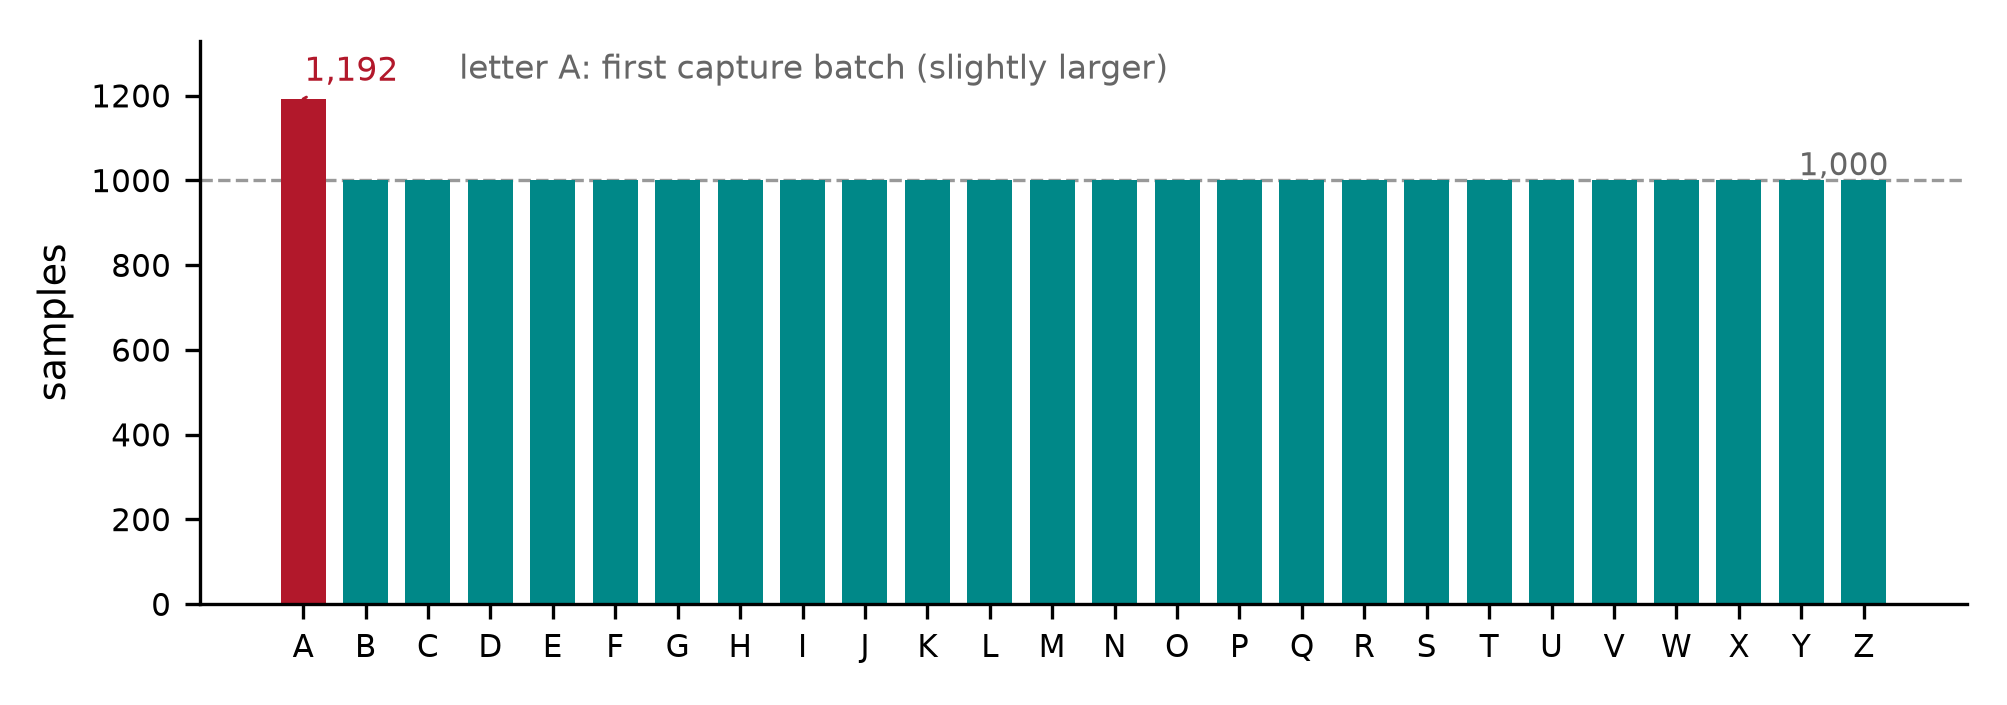
\includegraphics[width=0.86\textwidth]{figures/dataset_composition.png}
\caption{Dataset composition: 26,192 dual-hand samples across 26 letters
(letter~A = 1,192 from the first capture batch; B--Z = 1,000 each). The
stratified 85/15 split preserves these proportions in the 3,929-sample
test set.}
\label{fig:dataset}
\end{figure}

\begin{figure}[!htb]
\centering
\manualfig{A 3x2 grid of six real two-hand frames from the corpus, one per letter (A--F), each annotated with its letter label.}{Take six sample frames from the dataset (letters A to F), crop them to a consistent framing, arrange in 3 columns x 2 rows, and put a small letter badge in the corner of each tile. Same lighting/size across tiles.}
\caption{Sample frames from the dual-hand corpus (one per letter, A--F):
two-hand alphabet signs captured frontally with a laptop webcam.}
\label{fig:samples}
\end{figure}

Figure~\ref{fig:samples} shows six representative corpus frames;
Figure~\ref{fig:dataset} shows the per-letter counts. Letter~A carries
1,192 samples --- the first capture batch ran slightly longer before the
1,000-per-letter quota was fixed --- and every other letter carries
exactly 1,000. A stored sample is one frame: 84 landmark numbers
describing a single hand-pose snapshot, not a video clip. That
granularity keeps the dataset compact and matches the single-frame
recognizer the deployment needs; the stratified split then preserves
these proportions in the 3,929-sample test set, so no letter is judged
on a token sample.

The set is modest for production (captured by a small, homogeneous
group under similar conditions), so we regard the model as a strong
proof-of-concept, \emph{not yet production-ready}
(Section~\ref{sec:limitation}). For a short ablation only, we also
reference single-hand variants (63 features $(x,y,z)$ from one hand)
derived from a larger canonical capture stream; they are \emph{not}
deployed and only contextualize the accuracy--usability trade-off in
Section~\ref{sec:ablation}.

\subsection{Landmark Extraction}
\label{sec:landmarks}
MediaPipe Hands~\cite{mediapipehands2020} returns 21 landmarks per hand.
Analysis of the BISINDO alphabet shows 15 of 26 letters
(A, B, D, F, G, H, K, P, Q, R, S, T, W, X, Y) are predominantly two-handed,
and the remaining 11 (C, E, I, J, L, M, N, O, U, V, Z) single-handed.
This grouping is practical rather than purely linguistic: a few letters
(e.g., M, N, Q) are treated as single-handed because MediaPipe's
front-camera 2D view cannot reliably disambiguate their two-handed
articulations, so we adopt the representation the tracker captures
consistently. The system requests up to two hands. For dual-hand features
we keep $(x,y)$ and drop depth $z$, which is noisier across hands and
cameras; a missing second hand is zero-padded to a fixed length of 84.
Figure~\ref{fig:landmarks} plots two tracked hands from the corpus.

\begin{figure}[t]
\centering
\manualfig{Two real tracked hands with the MediaPipe skeleton overlay: 21 numbered landmarks per hand, wrist in red, fingertips in orange, connected in skeleton order.}{Best source: screenshot of the running app with the hand-overlay preview visible, signing a two-handed letter; tight crop, light background, at least 1600 px wide. Alternative: any MediaPipe Hands debug screenshot with two hands visible.}
\caption{Landmark extraction on two real tracked hands from the corpus:
21 anatomical landmarks per hand (wrist in red, fingertips in orange),
connected in skeleton order. Each hand yields 42 $(x,y)$ numbers; two
hands yield the 84 features used by the recognizer.}
\label{fig:landmarks}
\end{figure}

The landmark set is anatomically ordered: landmark~0 is the wrist,
1--4 run along the thumb, 5--8 the index finger, 9--12 the middle,
13--16 the ring, and 17--20 the little finger, so consecutive vector
positions are physically adjacent joints --- exactly the locality the
width-3 convolution exploits later (Section~\ref{sec:feature}). Keeping
$(x,y)$ per joint and dropping the noisy depth axis gives 42 numbers per
hand; a two-handed letter fills both 42-slot blocks and a single-handed
sign leaves the second block zero-padded.

\subsection{Three-Stage Normalization}
\label{sec:norm}
Raw coordinates depend on image position and camera distance. We apply (Fig.~\ref{fig:norm}):

\textbf{1) Wrist translation.} For each hand, subtract the wrist
(landmark 0):
\begin{equation}
\large
p_i' = p_i - p_0 .
\end{equation}

\textbf{2) Hand-size scaling.} Divide by the maximum Euclidean distance
from the wrist to any landmark of the same hand:
\begin{equation}
\large
\hat{p}_i = \frac{p_i'}{d_{\max}},\quad
d_{\max} = \max_j \|p_j - p_0\| .
\end{equation}

\textbf{3) Standardization.} A StandardScaler fitted on the training
split maps features to zero mean and unit variance; mean/scale vectors
are saved with the model for identical inference transforms. Zero-padded
absent-hand slots are left unchanged through normalization.
Figure~\ref{fig:normgeo} shows the first two stages on one real
two-hand frame.

\begin{figure}[t]
\centering
\manualfig{The same two-hand frame shown three times side by side: raw, after wrist translation, after hand-size scaling.}{Left panel: raw hands at different image positions and apparent sizes. Middle panel: both wrists pinned to the origin. Right panel: both hands at identical extent. Keep one hand teal and the other blue throughout; a small note mentions stage 3 (per-axis z-score).}
\caption{The first two normalization stages applied to one real
two-hand frame (teal = hand 1, blue = hand 2): raw hands differ in
position and apparent size; wrist translation pins both wrists to the
origin; hand-size scaling gives both hands identical extent. Stage~3
(per-axis z-score) then standardizes each axis using training-split
statistics only.}
\label{fig:normgeo}
\end{figure}

The raw hands sit at different image positions and different apparent
sizes --- depending on where, and how far from the camera, each signer
holds their hands. Translation pins both wrists to the origin and size
scaling gives both hands the same extent, after which the geometric
details that carry no sign information are gone; stage~3 then folds
each axis into zero-mean, unit-variance space using statistics fitted
on the training split only.

\begin{figure}[t]
\centering
\resizebox{0.58\textwidth}{!}{%
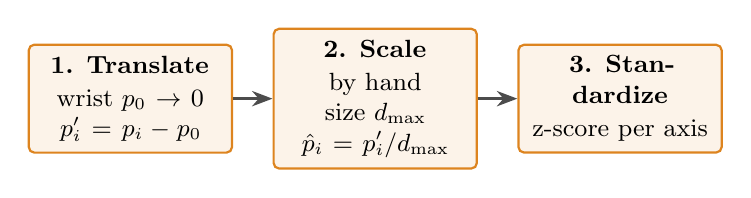
\begin{tikzpicture}[
  font=\small,
  node distance=4mm and 5mm,
  st/.style={rectangle, rounded corners=2pt, draw=cNorm, line width=0.8pt,
    fill=cNorm!10, align=center, inner sep=4pt, minimum height=12mm,
    text width=23mm},
  ar/.style={-{Stealth[length=2.6mm]}, line width=1pt, draw=black!70}]
\node[st] (n1) {\textbf{1. Translate}\\[1pt]wrist $p_0 \to 0$\\$p_i' = p_i - p_0$};
\node[st, right=of n1] (n2) {\textbf{2. Scale}\\[1pt]by hand size $d_{\max}$\\$\hat{p}_i = p_i'/d_{\max}$};
\node[st, right=of n2] (n3) {\textbf{3. Standardize}\\[1pt]z-score per axis};
\draw[ar] (n1) -- (n2);
\draw[ar] (n2) -- (n3);
\end{tikzpicture}}
\caption{Three-stage normalization: wrist translation, hand-size scaling,
and per-axis z-score standardization.}
\label{fig:norm}
\end{figure}

\subsection{Feature Representation}
\label{sec:feature}
After normalization, landmarks flatten to
\begin{equation}
\large
\mathbf{x} \in \mathbb{R}^{84}
= \big[\,\mathrm{hand}_1(x,y)_{0..20};\;
\mathrm{hand}_2(x,y)_{0..20}\,\big].
\end{equation}

This 84-vector is the sole input of the deployed model. The slot order
is fixed: landmarks 0--20 of the first detected hand occupy positions
0--41 and those of the second hand positions 42--83, in the same joint
order every frame. Fixed slots make zero-padding meaningful --- a
missing hand contributes an all-zero block that normalization leaves
untouched --- and give the convolution a predictable geometry: a width-3
kernel reads each joint with its immediate neighbours inside one hand,
except at the two block-boundary positions where kernels see both hands.
Single-hand ablations use $\mathbb{R}^{63}$ with $(x,y,z)$ on one hand
(Section~\ref{sec:ablation}).
Figure~\ref{fig:features} unpacks the vector.

\begin{figure}[!htb]
\centering
\manualfig{A flat 84-slot strip in two colored blocks: hand 1 (slots 0--41, teal) and hand 2 (slots 42--83, blue), one cell per landmark.}{Tick marks separate the cells; a dashed red line marks the block boundary between slots 41 and 42; one width-3 kernel window is highlighted inside hand 1 (joint + 2 neighbours, same hand), and the kernel crossing the boundary is marked as the only one that spans both hands.}
\caption{Anatomy of the 84-D input vector: two fixed 42-slot blocks,
one per hand, in a joint order that never changes between frames. A
width-3 kernel reads each joint with its two neighbours inside one
hand; only at the block boundary can a kernel span both hands.}
\label{fig:features}
\end{figure}

The 84 slots form two fixed 42-slot blocks, one per hand, in a joint
order that never changes between frames; the fixed semantics are what
make zero-padding meaningful and give the convolution a predictable
neighbourhood. A kernel centred on an interior joint reads that joint
and its two neighbours within the same hand; only at the single
boundary between the blocks can a kernel reach across hands. When only
one hand is present, the second block stays all zero through
normalization, so the model sees an unambiguous ``absent'' pattern
rather than noise.

\subsection{1D-CNN Architecture}
We use a three-block 1D-CNN suited to ordered landmark vectors
(Table~\ref{tab:arch}). Adaptive average pooling to length 1 yields a
fixed 64-D code regardless of input length, so the same head serves
dual-hand inputs. Total trainable parameters: 61{,}274.
Figure~\ref{fig:cnn-arch} traces the layer chain and the shrinking
tensor length through each pooling stage.

\begin{table}[t]
\caption{Deployed 1D-CNN (v1) for dual-hand 84-D input}
\label{tab:arch}
\centering
\begin{tabular}{ll}
\toprule
Layer & Configuration \\
\midrule
Input & $(1, 84)$ after channel reshape \\
Conv block 1 & 64 filt., $k{=}3$, pad 1, ReLU, MaxPool 2 \\
Conv block 2 & 128 filt., $k{=}3$, pad 1, ReLU, MaxPool 2 \\
Conv block 3 & 64 filt., $k{=}3$, pad 1, ReLU, AdaptiveAvgPool(1) \\
Flatten & 64 \\
FC 1 & $64\rightarrow128$, ReLU, Dropout 0.3 \\
FC 2 & $128\rightarrow26$ logits \\
Inference & Softmax over A--Z \\
\bottomrule
\end{tabular}
\end{table}

\begin{figure}[!htb]
\centering
\manualfig{Left-to-right layer chain: Input $1{\times}84$ -> Conv1 (64, $k{=}3$, ReLU, Pool 2 -> $64{\times}42$) -> Conv2 (128, $k{=}3$, ReLU, Pool 2 -> $128{\times}21$) -> Conv3 (64, $k{=}3$, ReLU, AAP(1) -> $64{\times}1$) -> Flatten 64 -> FC1 ($64{\to}128$, ReLU, Drop 0.3) -> FC2 ($128{\to}26$) -> Softmax A--Z.}{Draw the boxes in ONE straight row, simple arrows between them, no wrap-around connectors. Above the conv boxes add a shrinking bar ruler labelled: spatial length $84 \to 42 \to 21 \to 1$.}
\caption{Deployed \kw{1D-CNN} architecture (61{,}274 parameters): three
conv blocks with max-pooling, then \kw{adaptive average pooling} to a fixed
64-D code and two FC layers to 26 letter logits. Tensor length halves
at each pooling stage (ruler above).}
\label{fig:cnn-arch}
\end{figure}

Single-hand ablation checkpoints that report higher numeric accuracy used
a wider adaptive pool (flatten 512) and are not part of the deployed stack.

\subsection{Training Protocol}
\label{sec:train}
Optimization uses Adam (learning rate $0.001$), batch size 256, 50 epochs,
and cross-entropy loss; dropout is 0.3 and the scaler is fit only on the
training split. Artifacts saved per run: PyTorch weights, scaler JSON,
label map, and metrics JSON. Unless noted, deployed-model metrics are
confirmed by independent re-evaluation from the checkpoint with the same
split seed.
Figure~\ref{fig:twolane} separates the two phases.

\begin{figure}[!htb]
\centering
\manualfig{Two horizontal lanes --- OFFLINE (once, at training time) and ONLINE (every frame, in-browser) --- connected by one dashed cross-lane arrow.}{Offline lane: dual-hand dataset 26,192 -> 3-stage normalization (fit scaler) -> train 1D-CNN (61,274 params, 152.8 s CPU) -> export ONNX 241 KB. Online lane: MediaPipe Hands -> normalize (saved scaler) -> ONNX Runtime Web (0.53 ms mean) -> letter + sentence builder. Dashed arrow from ONNX export down into ONNX Runtime, labelled: same weights + scaler.}
\caption{Two phases of the deployed system: offline training (once) and
online inference (every frame, in-browser). Only the green lane runs
while a meeting is live.}
\label{fig:twolane}
\end{figure}

Everything expensive happens once, offline: fitting the scaler,
optimizing the 61,274 parameters, and exporting the graph. The online
lane repeats only cheap per-frame work --- landmark extraction, the
fixed normalization transform, and a 0.53~ms ONNX forward pass ---
inside the participant's browser tab. This split is why a meeting stays
live while recognition runs: no per-frame work depends on the training
pipeline.


% ============================================================
\section{Implementation}
\label{sec:impl}

\subsection{ONNX Browser Inference}
The dual-hand PyTorch checkpoint is exported with
\texttt{torch.onnx.export} (opset 12, dynamic batch). The artifact is
241~KB on disk (247{,}229 bytes) with input shape
$[\mathrm{batch},1,84]$ and 26-way output. In the browser we load
ONNX Runtime Web~\cite{onnx} version 1.17.1, apply the same three-stage
normalization via the saved scaler, and run softmax client-side.
Numerical parity versus PyTorch was verified with maximum absolute
difference below $4\times10^{-6}$. No frame or landmark leaves the device
for classification, supporting privacy-sensitive use.
Figure~\ref{fig:privacy} traces what crosses the network and what does
not.

\begin{figure}[!htb]
\centering
\manualfig{On-device recognition box (dotted boundary: camera -> MediaPipe -> ONNX) versus the server and peer browsers, with exactly two outbound arrows.}{Dashed arrow 1: letters/sentences (text events) from browser to Socket.IO server. Arrow 2: audio/video peer-to-peer from browser to peer browsers, bypassing the server. Small label under the browser box: 84 floats stay on-device.}
\caption{Network data flow. Recognition consumes 84 landmark numbers and
runs entirely on-device; the signaling server relays text events only,
and audio/video flows peer-to-peer over WebRTC without a media relay.}
\label{fig:privacy}
\end{figure}

A $640\times480$ frame carries roughly $9.2\times10^{5}$ pixel values,
yet recognition needs only 84 landmark numbers, and those never leave
the tab. What does leave is the composed text --- committed letters and
sentences over Socket.IO --- and the audio/video streams, which flow
peer-to-peer over WebRTC. The signaling server therefore never touches
a frame, a landmark, or a media packet; it only helps browsers find
each other.

\subsection{Sentence Builder}
Letters are not emitted every frame. A client-side builder commits a
letter only after the predicted class stays stable (default 500~ms).
Edit gestures use a hold threshold (default 2~s): a closed fist deletes
the last committed letter (backspace), an open palm clears the current
word. Word and sentence boundaries follow no-hand timers (default 2~s for
space, 4~s for sentence completion). Completed text can be spoken with
browser TTS (\texttt{id-ID}) and emitted as Socket.IO events
(\texttt{letter\_committed}, \texttt{space\_inserted},
\texttt{sentence\_completed}) for remote display.
Figure~\ref{fig:sentence-rules} summarizes the rule set.

A short walkthrough shows the defaults working together. The signer
holds B long enough to commit it, then I and N; a brief misread of U is
removed with a two-second fist; an open palm clears the current word if
needed; two seconds of empty hands insert a space, and four seconds end
the sentence, which TTS then speaks aloud. All thresholds are
configuration constants rather than learned parameters, so tuning
latency against misfire rate is a one-line change, not a retraining
cycle.

\begin{figure}[!htb]
\centering
\resizebox{0.555\textwidth}{!}{%
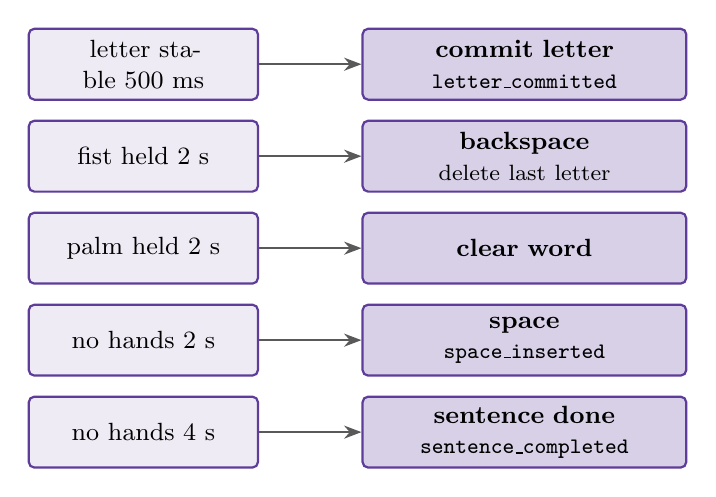
\begin{tikzpicture}[
  font=\small,
  cond/.style={rectangle, rounded corners=2pt, draw=cLogic, line width=0.8pt,
    fill=cLogic!10, text=black, align=center, minimum height=9mm,
    inner sep=3pt, text width=27mm},
  outc/.style={rectangle, rounded corners=2pt, draw=cLogic, line width=0.8pt,
    fill=cLogic!24, text=black, align=center, minimum height=9mm,
    inner sep=3pt, text width=39mm},
  rule/.style={-{Stealth[length=2.2mm]}, line width=0.9pt, draw=black!65},
  node distance=2.4mm and 13mm,
]
\node[cond] (c1) {letter stable 500~ms};
\node[cond, below=of c1] (c2) {fist held 2~s};
\node[cond, below=of c2] (c3) {palm held 2~s};
\node[cond, below=of c3] (c4) {no hands 2~s};
\node[cond, below=of c4] (c5) {no hands 4~s};
\node[outc, right=of c1] (o1) {\kw{commit letter}\\\footnotesize\texttt{letter\_committed}};
\node[outc, right=of c2] (o2) {\kw{backspace}\\\footnotesize delete last letter};
\node[outc, right=of c3] (o3) {\kw{clear word}};
\node[outc, right=of c4] (o4) {\kw{space}\\\footnotesize\texttt{space\_inserted}};
\node[outc, right=of c5] (o5) {\kw{sentence done}\\\footnotesize\texttt{sentence\_completed}};
\draw[rule] (c1.east) -- (o1.west);
\draw[rule] (c2.east) -- (o2.west);
\draw[rule] (c3.east) -- (o3.west);
\draw[rule] (c4.east) -- (o4.west);
\draw[rule] (c5.east) -- (o5.west);
\end{tikzpicture}}
\caption{Sentence-builder rules: stability commit, fist/palm edit
gestures, and no-hand timers for word and sentence boundaries.}
\label{fig:sentence-rules}
\end{figure}

\subsection{Meeting Architecture}
\label{sec:meeting-arch}
Figure~\ref{fig:meeting} shows the collaboration design. Media flows
full-mesh over WebRTC among peers, simple to deploy but poorly scaling: a
room of $n$ participants requires each peer to maintain $n-1$ outbound
media streams, an $O(n^2)$ total connection cost, acceptable for small
rooms but a bottleneck as $n$ grows (Section~\ref{sec:runtime}). The
Flask-SocketIO server performs room membership and SDP/ICE signaling only;
it does not relay video. Google STUN is always available for NAT
traversal; a public best-effort TURN (Metered openrelay) serves as a
client-side fallback, and an optional self-hosted TURN can be supplied at
runtime via \texttt{/api/turn} so credentials are never hard-coded in
static assets. Our deployment provisions no dedicated TURN (the host
sits behind consumer NAT), so we rely on the public STUN/TURN path; a
media-relaying SFU is future work.

\begin{figure}[!htb]
\centering
\manualfig{Four peers P1-P4 in a square, fully interconnected (6 bidirectional media links, $O(n^2)$), plus a signaling-only server and STUN/TURN boxes.}{Solid red lines = media, full mesh, every pair of peers, bidirectional (6 links for n=4). Dashed lines = signaling: each peer to the Flask-Socket.IO server, and peers querying Google STUN / TURN for NAT traversal. Legend: media (P2P, $O(n^2)$) vs signaling (SDP/ICE).}
\caption{Meeting architecture: bidirectional full-mesh WebRTC media
($O(n^2)$; six links for $n{=}4$) with a \kw{signaling-only}
Flask--Socket.IO server; peers query STUN/TURN for NAT traversal.}
\label{fig:meeting}
\end{figure}

\subsection{Reliability Fixes}
Early multi-peer tests exposed three failure modes, each addressed:
\begin{itemize}
\item \textbf{Black/partial video under restrictive NAT} (CGNAT, campus
WiFi; STUN-only sessions) $\rightarrow$ public best-effort TURN fallback.
\item \textbf{Video dead after transient ICE drops} $\rightarrow$
automatic ICE restart with a guarded full reconnect on failure.
\item \textbf{Join races leaving existing peers uncontacted} $\rightarrow$
proactive connections from each joiner to every existing member, with
deterministic offer polarity by session id.
\end{itemize}

These fixes improve connection establishment and recovery in small
internal sessions but do \emph{not} remove the fundamental mesh scaling
limit: each peer uploads a separate stream to every other peer, so
sessions degrade asymmetrically as the room grows
(Section~\ref{sec:runtime}). Automated HTTPS smoke checks against the
deployed tunnel return HTTP~200 for the meeting shell, health/stats
APIs, ONNX assets (\texttt{model.onnx} 247{,}229~B, scaler, labels), and
client scripts.

\begin{figure}[t]
\centering
\begin{subfigure}[t]{\textwidth}
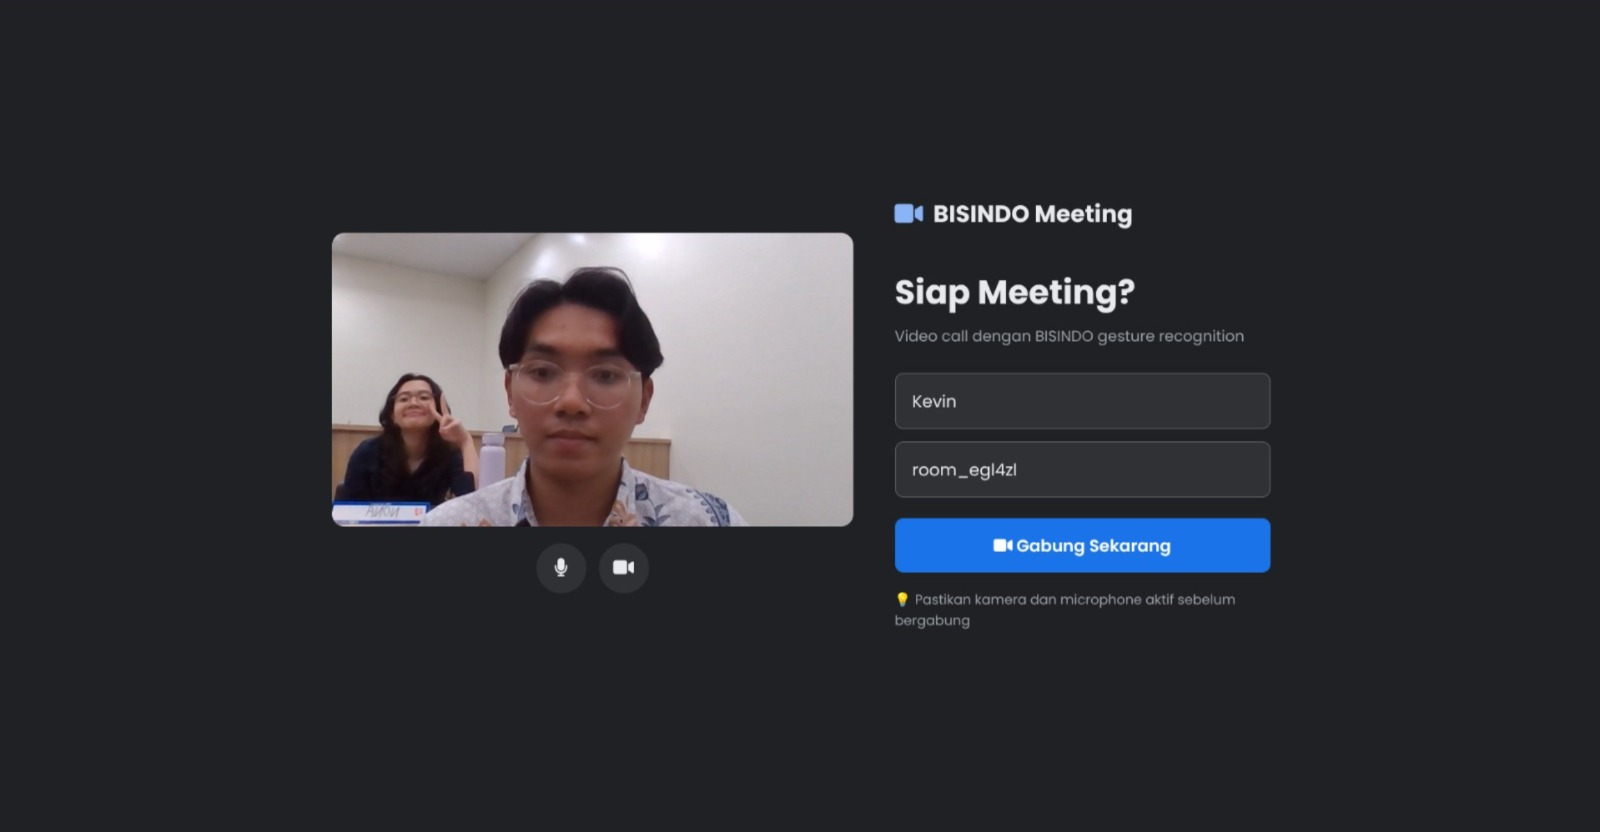
\includegraphics[width=\linewidth]{figures/eval-screenshots/01-lobby-join.jpeg}
\caption{Pre-join lobby with camera preview.}
\label{fig:ui-lobby}
\end{subfigure}

\vspace{3pt}

\begin{subfigure}[t]{\textwidth}
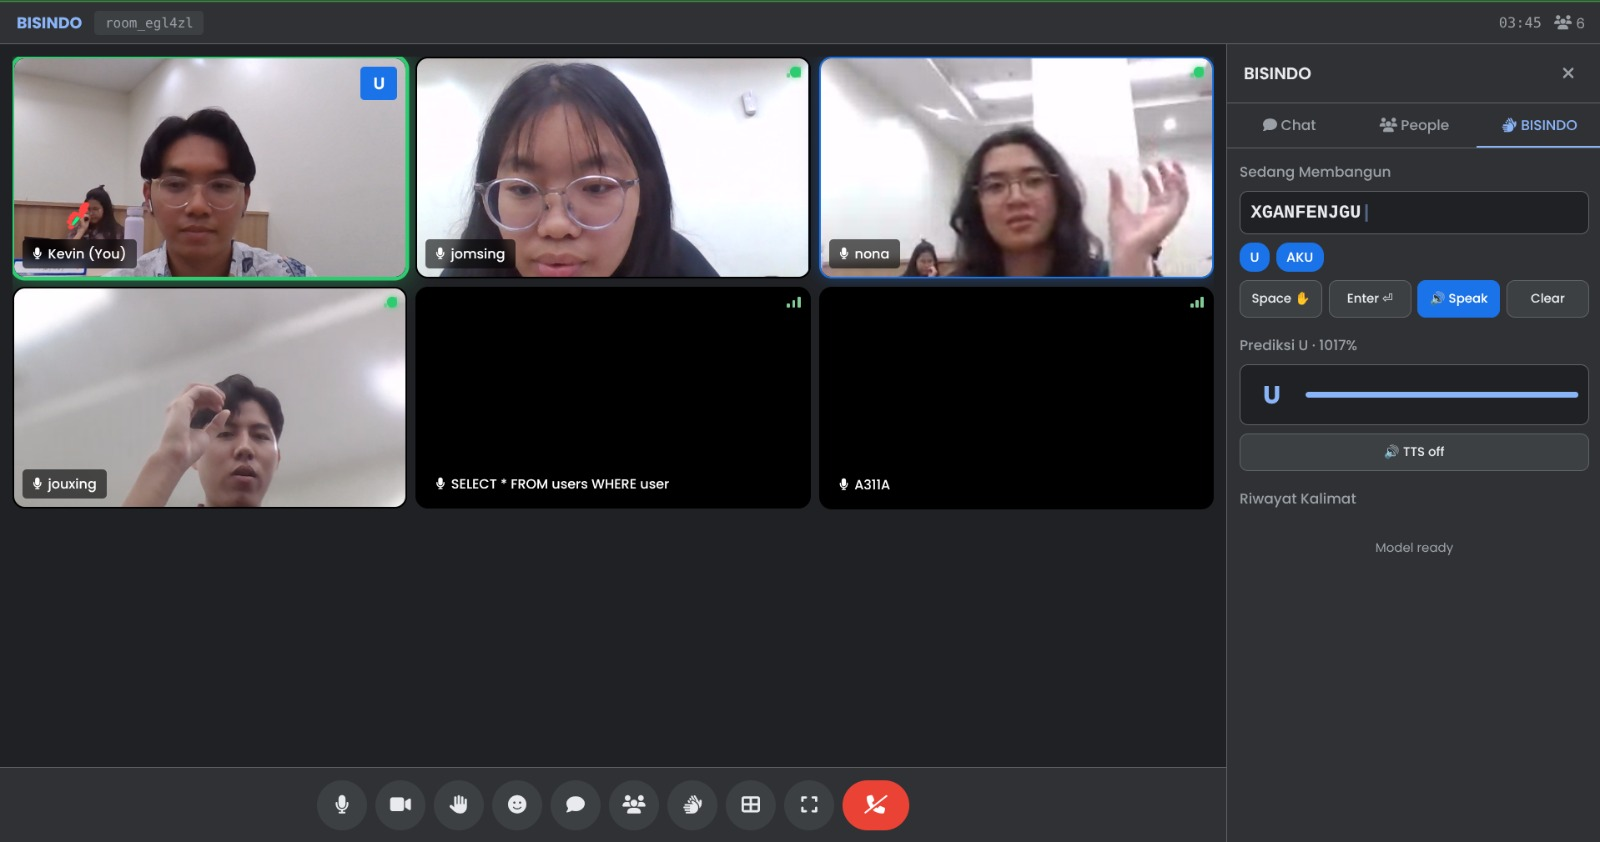
\includegraphics[width=\linewidth]{figures/eval-screenshots/03-letter-detection.jpeg}
\caption{Live letter composition panel.}
\label{fig:ui-letters}
\end{subfigure}
\caption{Client UI: (a)~pre-join lobby; (b)~live letter composition with
confidence readout.}
\label{fig:ui-functional}
\end{figure}

\begin{figure}[t]
\centering
\resizebox{0.52\textwidth}{!}{%
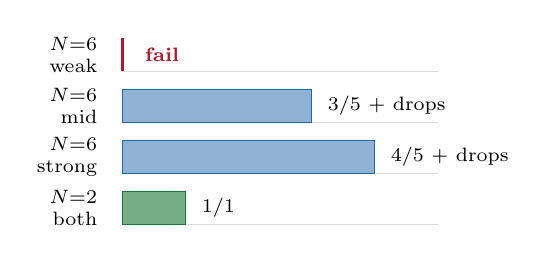
\begin{tikzpicture}[font=\scriptsize, x=1mm, y=1mm]
% 1 stream = 8 mm; max 5 streams = 40 mm
\foreach \i in {0,...,3} { \draw[black!15, line width=0.4pt] (0,\i*6.5) -- (40,\i*6.5); }
\draw[fill=cNet!60, draw=cNet, line width=0.5pt]   (0,0)    rectangle (8,4.2);
\draw[fill=cCapture!50, draw=cCapture, line width=0.5pt] (0,6.5)  rectangle (32,10.7);
\draw[fill=cCapture!50, draw=cCapture, line width=0.5pt] (0,13)   rectangle (24,17.2);
\draw[cModel, line width=1.2pt] (0,19.5) -- +(0,4.2);
\node[cModel, font=\scriptsize\bfseries] at (5,21.6) {fail};
\node[right, font=\scriptsize] at (8.8,2.1)   {1/1};
\node[right, font=\scriptsize] at (32.8,8.6)  {4/5 + drops};
\node[right, font=\scriptsize] at (24.8,15.1) {3/5 + drops};
\node[left, font=\scriptsize, align=right] at (-2,2.1)   {$N{=}2$\\both};
\node[left, font=\scriptsize, align=right] at (-2,8.6)   {$N{=}6$\\strong};
\node[left, font=\scriptsize, align=right] at (-2,15.1)  {$N{=}6$\\mid};
\node[left, font=\scriptsize, align=right] at (-2,21.6)  {$N{=}6$\\weak};
\end{tikzpicture}}
\caption{Full-mesh reception from Table~\ref{tab:scalability}: remote
streams rendered (of $N{-}1$) per observer in the live session.
Reception is asymmetric and collapses entirely on the weak (cellular)
uplink.}
\label{fig:mesh-chart}
\end{figure}

\subsection{Deployment Footprint}
A static web demo (capture and offline test pages) suits static hosting
(e.g., Vercel). The meeting service runs as a lightweight local
Flask-SocketIO process on a commodity laptop (Intel Core Ultra 5 125U,
14 logical cores, no GPU); public HTTPS ingress uses a Cloudflare quick
tunnel, so the host need not expose inbound media ports or a public IP.
Quick-tunnel URLs are ephemeral and change on restart; a named tunnel is
planned for stable public demos. The small footprint follows from the
architecture rather than from a post-hoc optimization: the model ships
inside the web bundle, so the server process holds no weights and spends
its budget on signaling alone, and the $O(n^2)$ media fan-out of the
mesh lands on the participants' uplinks rather than on the host
(Section~\ref{sec:syseval}). The same commodity laptop serves training,
inference testing, and the meeting itself, which is what makes
single-machine demonstrations and repeated redeployment during
development practical.
% PLACEHOLDER: named-tunnel — production named Cloudflare tunnel hostname


% ============================================================
\section{Experiments}
\label{sec:experiments}

\subsection{Setup}
Training used PyTorch on CPU (Intel Core Ultra 5 125U, 14 logical
cores, 30~GB RAM; no GPU) with the protocol in
Section~\ref{sec:train}; dual-hand training completed in 152.8~s wall
time. Metrics are accuracy, weighted F1, and per-class
precision/recall/F1 (scikit-learn). The dual-hand test set has
3{,}929 samples (stratified 15\%, seed 42). Deployment checks used Chrome
with MediaPipe Hand Landmarker (float16) and ONNX Runtime Web 1.17.1. The
meeting service runs as a local Flask-SocketIO process (signaling only)
over a Cloudflare quick tunnel; recognition stays on-device in each browser.

\subsection{Evaluation Metrics}
\label{sec:metrics}
We report accuracy, weighted F1, and per-class precision, recall, and
F1, computed with scikit-learn on the held-out test set ($n{=}3{,}929$).
Accuracy alone can hide class-level failures: a model can be 98\% correct
and still miss one letter consistently, which matters here because every
wrong or missed letter enters the sentence the deaf participant is
composing. Per-class precision (how often a predicted letter is right)
and recall (how often a true letter is caught) expose exactly that.
Weighted F1 averages per-class F1 with support as the weights; because
the stratified split keeps classes nearly equal at about 150 test
samples per letter, weighted and macro F1 nearly coincide here, and the
weighted F1 (98.45\%) matching the accuracy confirms the model does not
lean on frequent classes. The classifier head is a softmax over the 26
letters, trained with categorical cross-entropy.

\begin{figure}[t]
\centering
\resizebox{0.49\textwidth}{!}{%
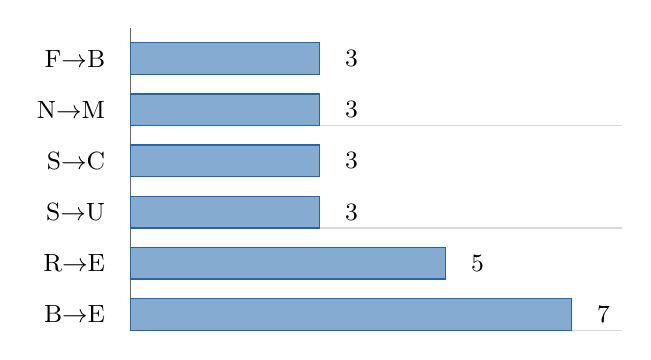
\begin{tikzpicture}[font=\small, x=8mm, y=6.5mm]
\foreach \i in {0,2,4} { \draw[black!15, line width=0.4pt] (0,\i) -- (7.8,\i); }
\draw[black!60, line width=0.5pt] (0,0) -- (0,5.9);
\foreach \y/\w/\l in {0.0/7/B$\to$E, 1.0/5/R$\to$E, 2.0/3/S$\to$U,
                      3.0/3/S$\to$C, 4.0/3/N$\to$M, 5.0/3/F$\to$B} {
  \draw[fill=cCapture!55, draw=cCapture, line width=0.5pt]
    (0,\y) rectangle (\w,{\y+0.62});
  \node[right, font=\small] at ({\w+0.25},{\y+0.31}) {\w};
  \node[left,  font=\small] at (-0.25,{\y+0.31}) {\l};
}
\end{tikzpicture}}
\caption{Most frequent misclassifications of the dual-hand model
(true $\rightarrow$ predicted, test set $n{=}3{,}929$).}
\label{fig:confusions}
\end{figure}

\subsection{Main Result: Dual-Hand Model}
The deployed dual-hand model reaches \textbf{98.45\% accuracy} and
\textbf{98.45\% weighted F1}, independently re-evaluated from the saved
checkpoint: 3{,}868 of 3{,}929 held-out samples are correct, and the 61
residual errors cluster on visually similar letters
(Fig.~\ref{fig:confusions}; full matrix in Fig.~\ref{fig:confmat}).
Full per-class metrics are in
Table~\ref{tab:perclass} and Fig.~\ref{fig:perclass}; the hardest
letters are B (0.94 F1), E (0.96), and F (0.97), consistent with
overlapping finger configurations. The floor matters as much as the
average: every one of the 26 letters scores at least 0.94~F1, so no
letter fails consistently --- the failure mode that would silently
corrupt every word containing it. Expressed differently, about one
test frame in 65 is misclassified, and the residual errors concentrate
on letter pairs a human observer would also confuse rather than being
spread over random classes.

\begin{table}[t]
\caption{Per-class performance -- dual-hand model (re-evaluated, $n{=}3929$)}
\label{tab:perclass}
\centering
\setlength{\tabcolsep}{5pt}
\begin{tabular}{lcccc@{\hspace{14pt}}lcccc}
\toprule
L & P & R & F1 & Sup & L & P & R & F1 & Sup \\
\midrule
A & .994 & .994 & .994 & 179 & N & .980 & .967 & .973 & 150 \\
B & .952 & .933 & .943 & 150 & O & .993 & .993 & .993 & 150 \\
C & .974 & .993 & .984 & 150 & P & .980 & 1.00 & .990 & 150 \\
D & 1.00 & .980 & .990 & 150 & Q & .993 & 1.00 & .997 & 150 \\
E & .926 & 1.00 & .962 & 150 & R & .993 & .967 & .980 & 150 \\
F & .986 & .953 & .970 & 150 & S & 1.00 & .960 & .980 & 150 \\
G & .993 & 1.00 & .997 & 150 & T & .993 & .993 & .993 & 150 \\
H & 1.00 & 1.00 & 1.00 & 150 & U & .955 & .993 & .974 & 150 \\
I & .961 & .980 & .970 & 150 & V & 1.00 & .987 & .993 & 150 \\
J & .993 & 1.00 & .997 & 150 & W & .993 & 1.00 & .997 & 150 \\
K & 1.00 & .987 & .993 & 150 & X & .987 & .973 & .980 & 150 \\
L & 1.00 & 1.00 & 1.00 & 150 & Y & .987 & .987 & .987 & 150 \\
M & .967 & .973 & .970 & 150 & Z & 1.00 & .980 & .990 & 150 \\
\bottomrule
\end{tabular}
\end{table}

\begin{figure}[t]
\centering

\includegraphics[width=0.84\textwidth]{figures/cnn_2hand_per_class_chart.png}
\caption{Per-class precision, recall, and F1 (dual-hand model). Most
letters exceed 0.97 F1; hardest are B, E, and F.}
\label{fig:perclass}
\end{figure}
\begin{figure}[t]
\centering
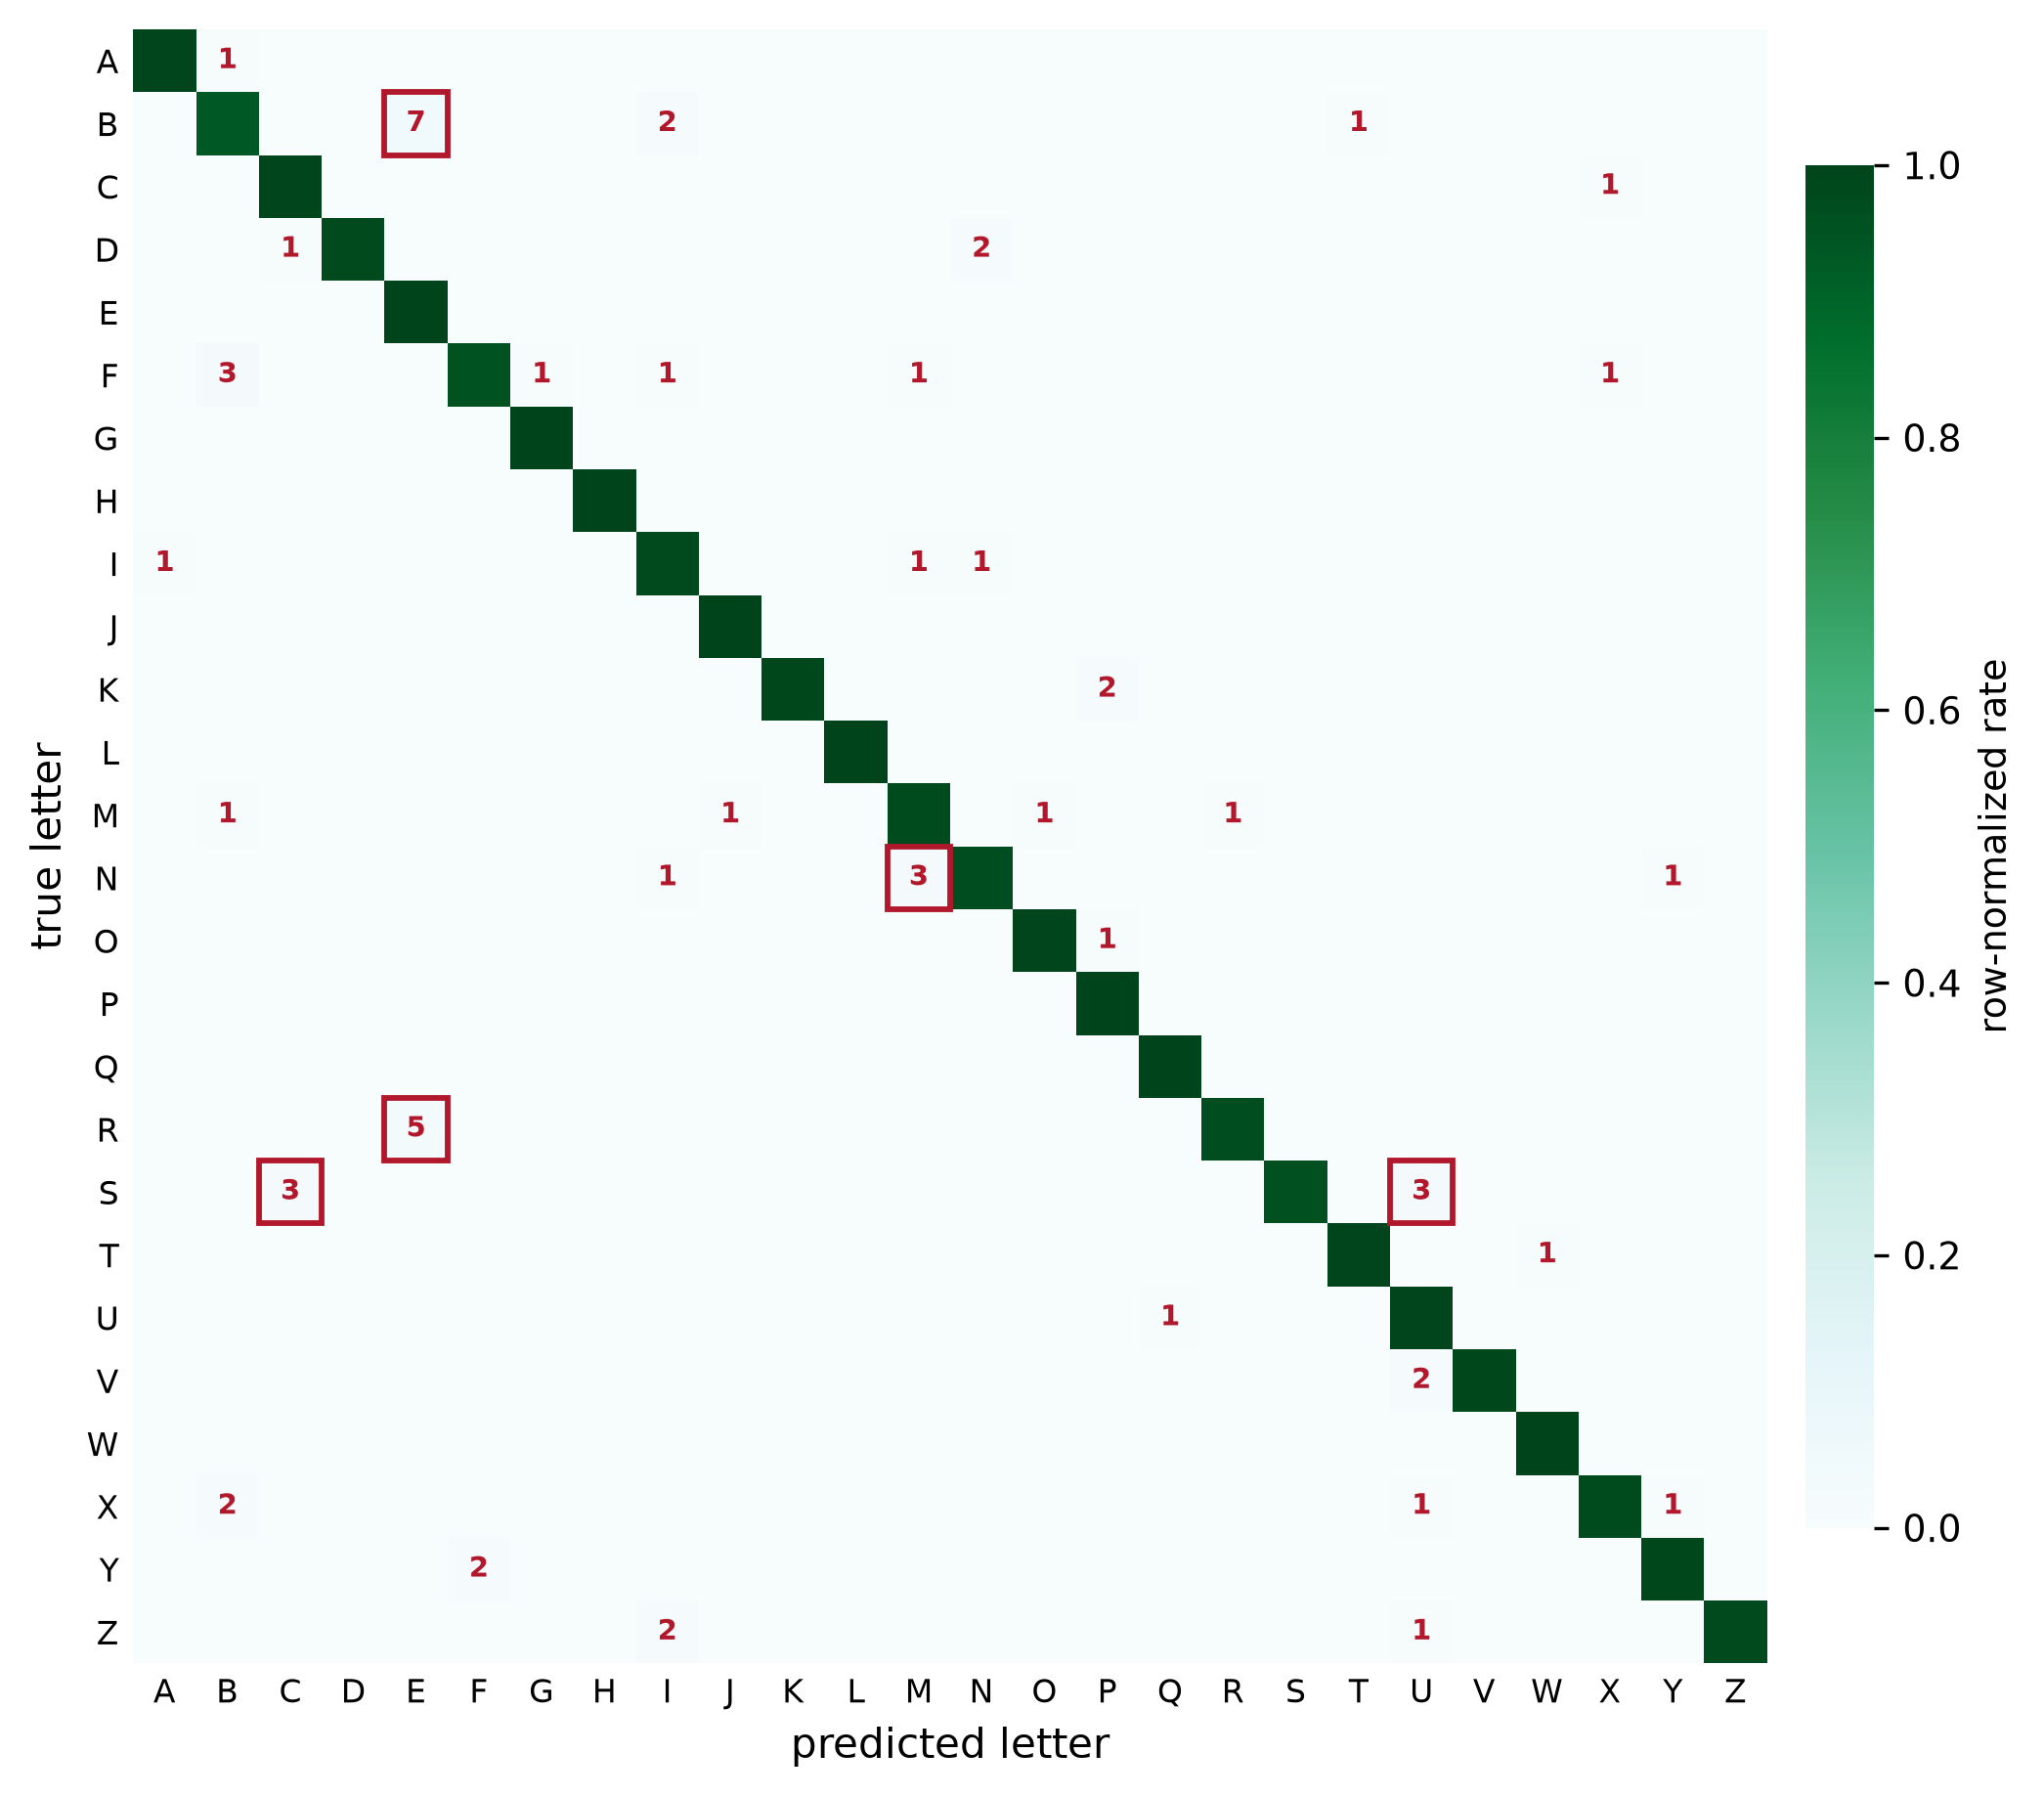
\includegraphics[width=0.72\textwidth]{figures/confusion_2hand_clean.png}
\caption{Confusion matrix of the deployed dual-hand model ($n{=}3{,}929$,
row-normalized shading; off-diagonal counts annotated). Only 61 of
3{,}929 frames are misclassified; the five most confusable pairs
(B$\to$E, R$\to$E, S$\to$U, S$\to$C, N$\to$M, boxed) account for 21 of
them and are all visually similar handshapes.}
\label{fig:confmat}
\end{figure}


\subsection{Compact Ablation: Why Not Single-Hand?}
\label{sec:ablation}
Table~\ref{tab:ablation} contrasts the deployed dual-hand model with
two single-hand references trained on the larger canonical capture
stream. The balanced single-hand model posts the highest number,
99.12\%, but the comparison is not as simple as the numbers suggest. A
single-hand model sees one hand, so letters that require both --- most
of the BISINDO alphabet in our grouping
(Section~\ref{sec:landmarks}) --- fall outside what it can ever
recognize; its 99.12\% applies to that restricted input world. The
deployed dual-hand model accepts both hands and covers all 26 letters in
one model, at a cost of 0.67 percentage points against the balanced
reference. For a communication tool that must accept whatever a signer
does, coverage is the point, so we deploy the dual-hand model and report
its honest 98.45\%.

\begin{table}[t]
\caption{Ablation: single-hand vs.\ deployed dual-hand}
\label{tab:ablation}
\centering
\begin{tabular}{@{}lccc l@{}}
\toprule
Model & Feat. & Hands & Acc. & Note \\
\midrule
Baseline (1H) & 63 & 1 & 96.04\% & ref. \\
Balanced (1H) & 63 & 1 & 99.12\% & best acc.\dag \\
\textbf{2Hand} & \textbf{84} & \textbf{2} & \textbf{98.45\%} & \textbf{deployed}\ddag \\
\bottomrule
\multicolumn{5}{@{}l@{}}{\footnotesize\dag{} training-time metric; not deployed (1-hand only).}\\
\multicolumn{5}{@{}l@{}}{\footnotesize\ddag{} independently re-evaluated.}\\
\end{tabular}
\end{table}

\subsection{Runtime and Product Checks}
\label{sec:runtime}
The deployed classifier is small (61{,}274 parameters, 241~KB ONNX), so
classifier-only inference runs far above real-time; the full
in-browser pipeline is dominated by MediaPipe landmark detection, not
ONNX inference. Over 2{,}000 single-vector
($1\times1\times84$) inferences with ONNX Runtime on CPU (14 threads
available), classifier-only latency is \textbf{0.53~ms mean / 0.31~ms
median / 1.21~ms P95} ($\approx$1{,}870 inferences/s), confirming the
recognition head is not the bottleneck.
Figure~\ref{fig:latency} breaks the per-frame cost down and summarizes the
calibrated frame rate measured in Section~\ref{sec:syseval}.
% latency-browser-e2e: measured 2026 — full pipeline + broadcast figures in Section~\ref{sec:syseval}

\begin{figure}[t]
\centering
\begin{subfigure}[t]{0.58\linewidth}
\centering
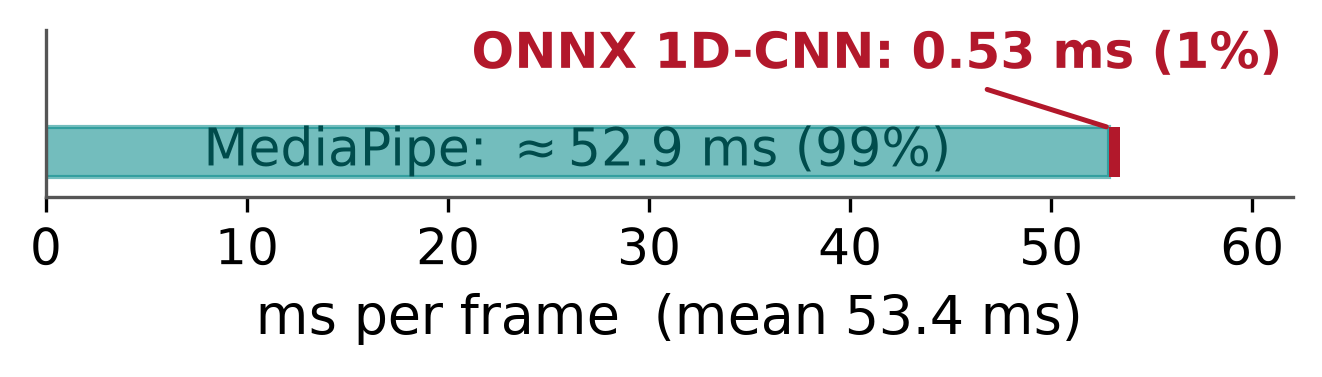
\includegraphics[width=\linewidth]{figures/latency_cost.png}
\caption{Per-frame cost (53.4~ms mean).}
\label{fig:latency-breakdown}
\end{subfigure}%
\hfill
\begin{subfigure}[t]{0.33\linewidth}
\centering
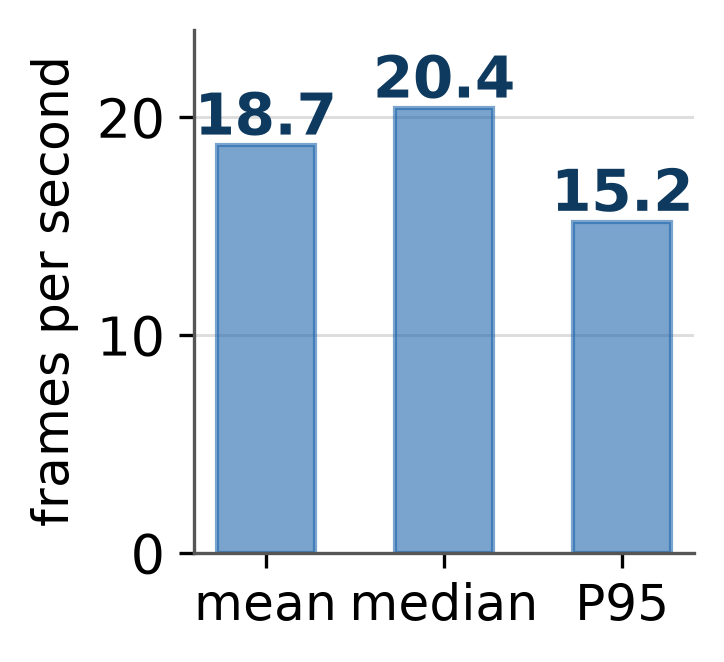
\includegraphics[width=\linewidth]{figures/latency_fps.png}
\caption{Frame rate (FPS).}
\label{fig:latency-fps}
\end{subfigure}
\caption{Browser pipeline latency and frame rate (100 frames,
640$\times$480): ONNX inference is $\approx$1\% of a frame; MediaPipe
landmark detection dominates.}
\label{fig:latency}
\end{figure}

The meeting stack is served locally behind a Cloudflare quick tunnel;
public HTTPS checks return \texttt{status=ok}, serve the dual-hand ONNX
bundle (241~KB), and load client scripts. Functional multi-user sessions
confirmed the recognition overlay, live sentence broadcast, and recovery
after transient network blips following the reliability fixes in
Section~\ref{sec:impl}. Figure~\ref{fig:ui-functional} shows the pre-join
lobby and the in-meeting recognition panel composing letters live.
No formal deaf-community user study is claimed here.

% PLACEHOLDER: user-study — optional N-user task success rates

\subsection{System Evaluation (Mesh Scalability)}
\label{sec:syseval}
Because media uses a full mesh, per-peer upstream load grows with room
size. To characterize the deployed system's practical ceiling, we
ran controlled multi-participant sessions, recording for each observer
how many of the other $n-1$ remote streams rendered and
whether frame drops occurred (Table~\ref{tab:scalability},
Fig.~\ref{fig:mesh-chart}). Reception is
\emph{asymmetric}: participants on stronger uplinks receive all peers, while
those on weaker links receive only a subset, with degradation pronounced
beyond a small room size. Concretely (Table~\ref{tab:scalability}): with
two participants the mesh behaves like a direct call and everyone
receives everything; at six, a strong-uplink observer still renders 4 of
5 streams, a mid-link observer 3 of 5, and a cellular-uplink observer
fails to join usefully at all. The gap between strong and weak
participants is the practical cost of $O(n^2)$ media without a relay,
and it is the single clearest argument for the SFU listed as future
work.
% PLACEHOLDER: scalability data — fill after re-running the N-peer test.
%   Columns: N participants | observer | streams received (of N-1) |
%   frame drops (y/n) | device / uplink. Repeat for N=2..5.

\begin{table}[t]
\caption{Full-mesh reception vs.\ room size (live observation).
``Recv.'' counts how many of the $N{-}1$ remote streams rendered;
--- = not recorded (the weak peer failed to join).}
\label{tab:scalability}
\centering
\setlength{\tabcolsep}{4pt}
\begin{tabular}{@{}clccl@{}}
\toprule
$N$ & Observer & Recv. & Drops & Uplink \\
\midrule
2 & both    & 1/1  & no  & laptop / Wi-Fi \\
6 & strong  & 4/5  & yes & laptop / Wi-Fi \\
6 & mid     & 3/5  & yes & mixed \\
6 & weak    & fail & --- & mobile / cellular \\
\bottomrule
\end{tabular}
\end{table}


\begin{figure}[!htb]
\centering
\begin{subfigure}[t]{0.38\textwidth}
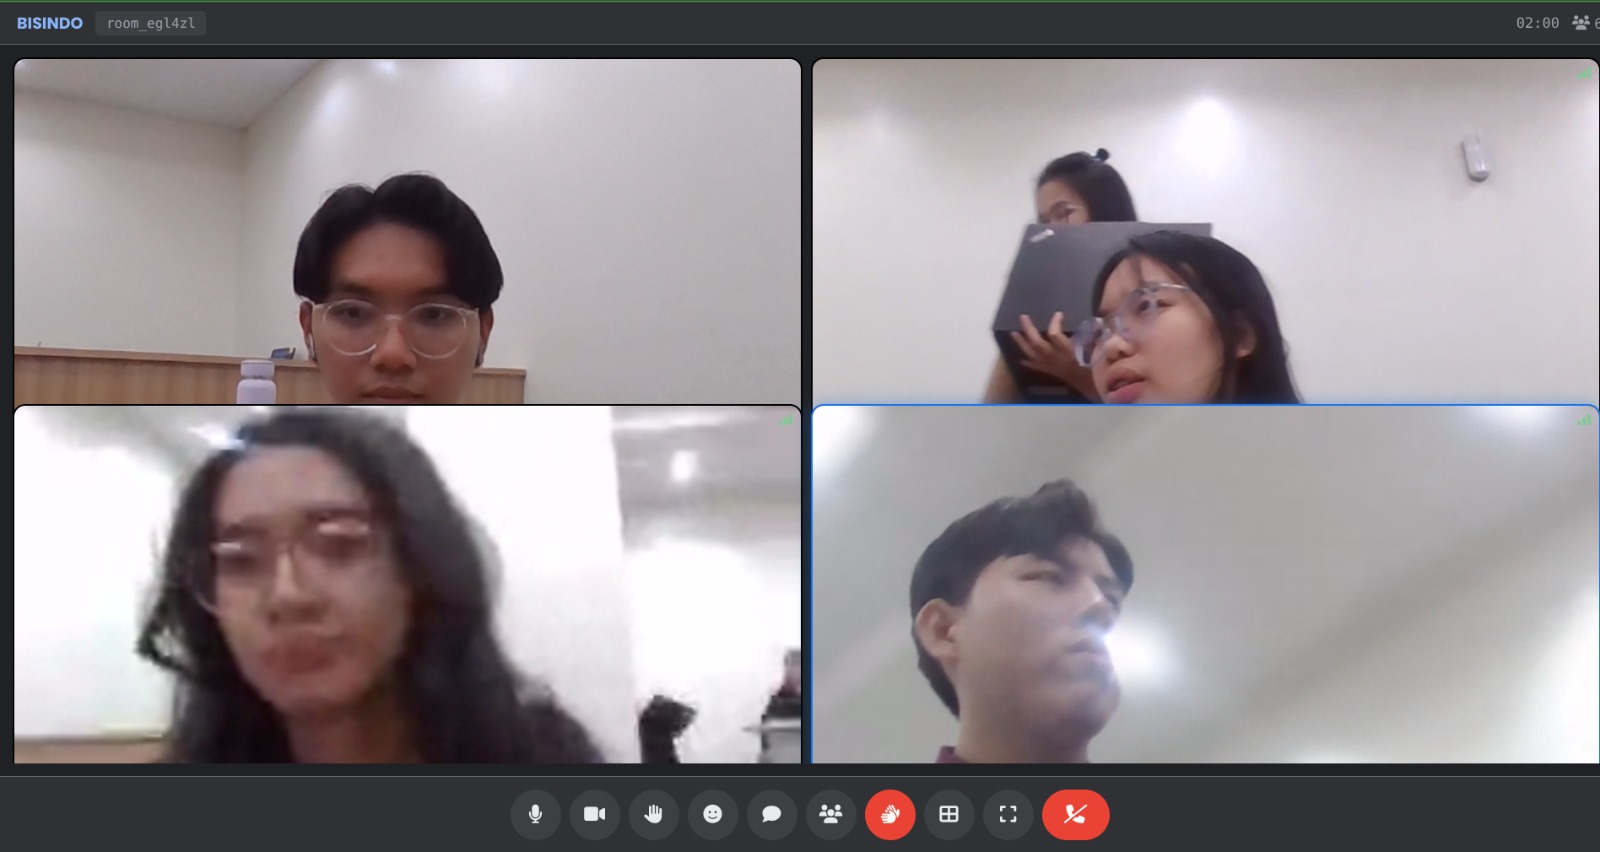
\includegraphics[width=\linewidth]{figures/eval-screenshots/02-normal-4tiles.jpeg}
\caption{Baseline: all tiles render.}
\label{fig:mesh-normal}
\end{subfigure}%
\hfill
\begin{subfigure}[t]{0.38\textwidth}
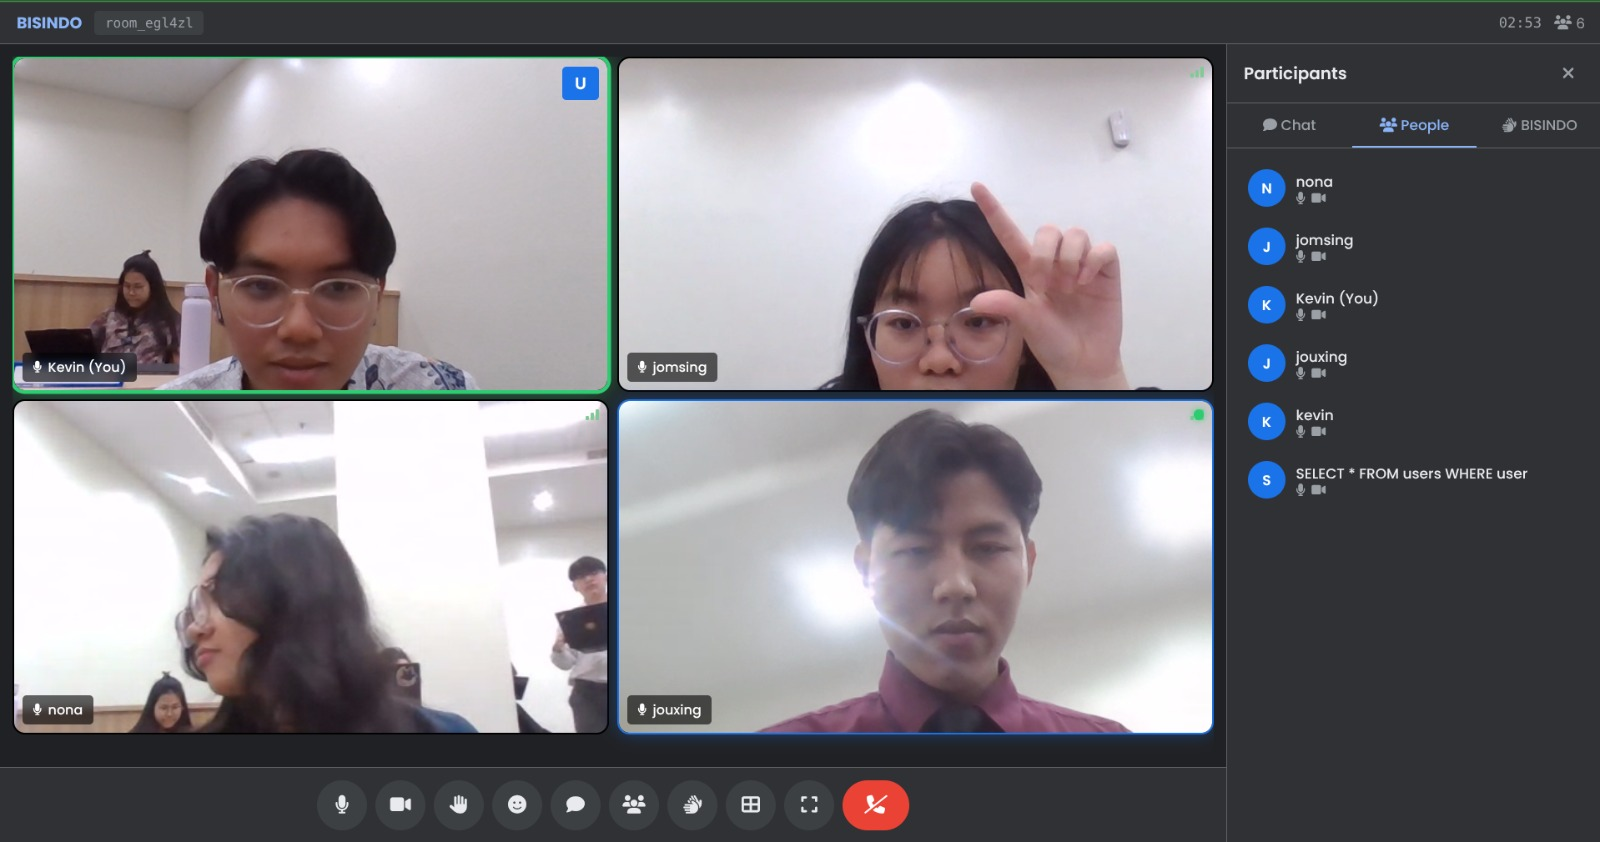
\includegraphics[width=\linewidth]{figures/eval-screenshots/04-mesh-6joined-4shown.jpeg}
\caption{Roster reports 6, only 4 render.}
\label{fig:mesh-count}
\end{subfigure}

\vspace{6pt}

\begin{subfigure}[t]{0.38\textwidth}
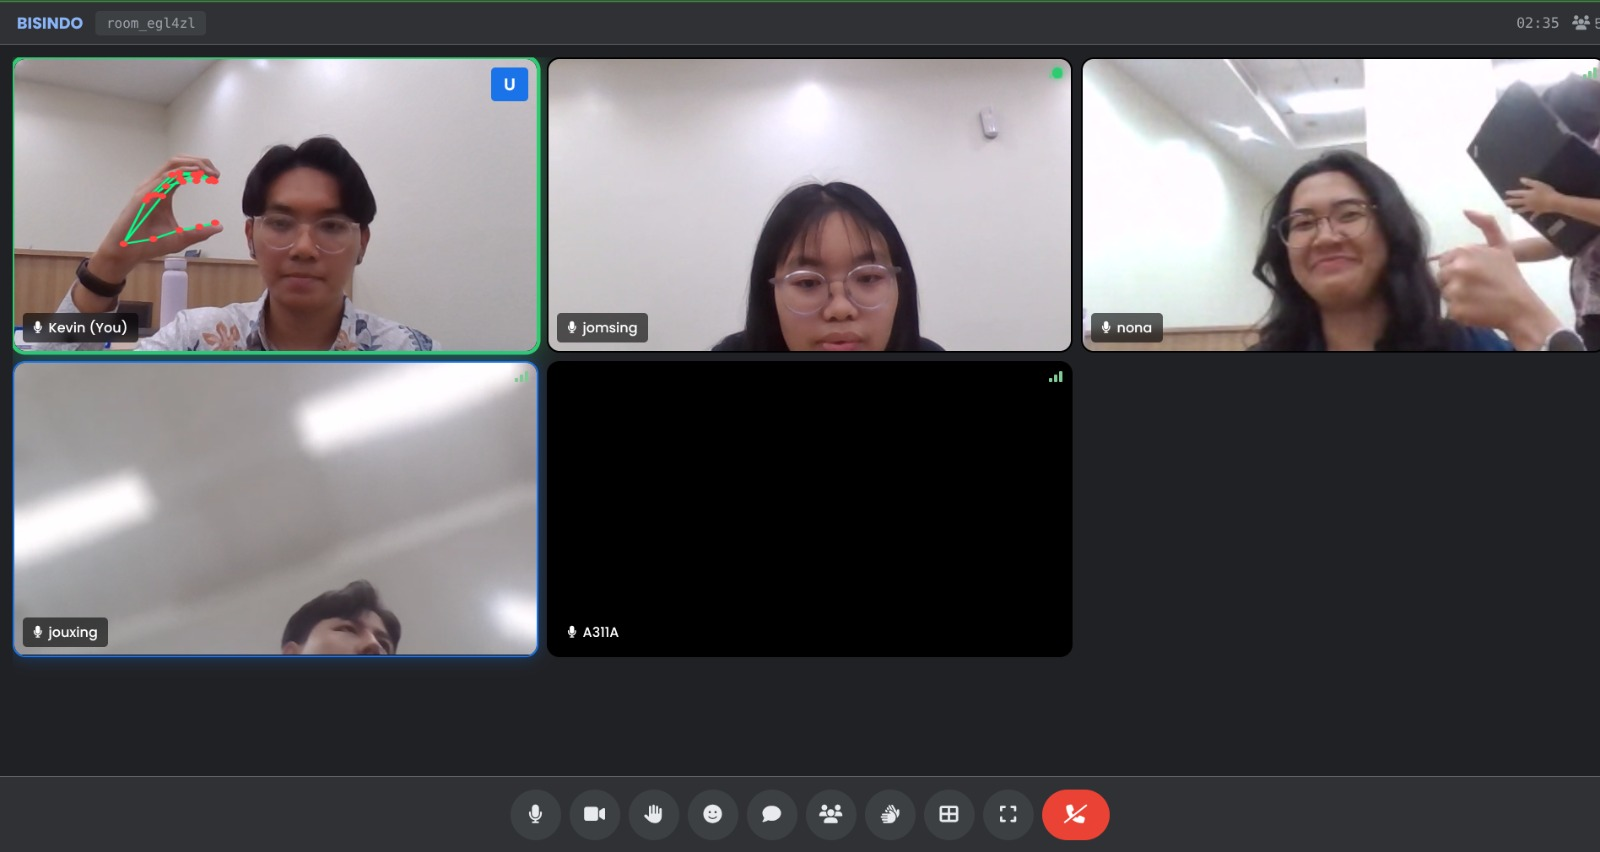
\includegraphics[width=\linewidth]{figures/eval-screenshots/05-black-tile-bug.jpeg}
\caption{Black / frozen tiles.}
\label{fig:mesh-black}
\end{subfigure}%
\hfill
\begin{subfigure}[t]{0.38\textwidth}
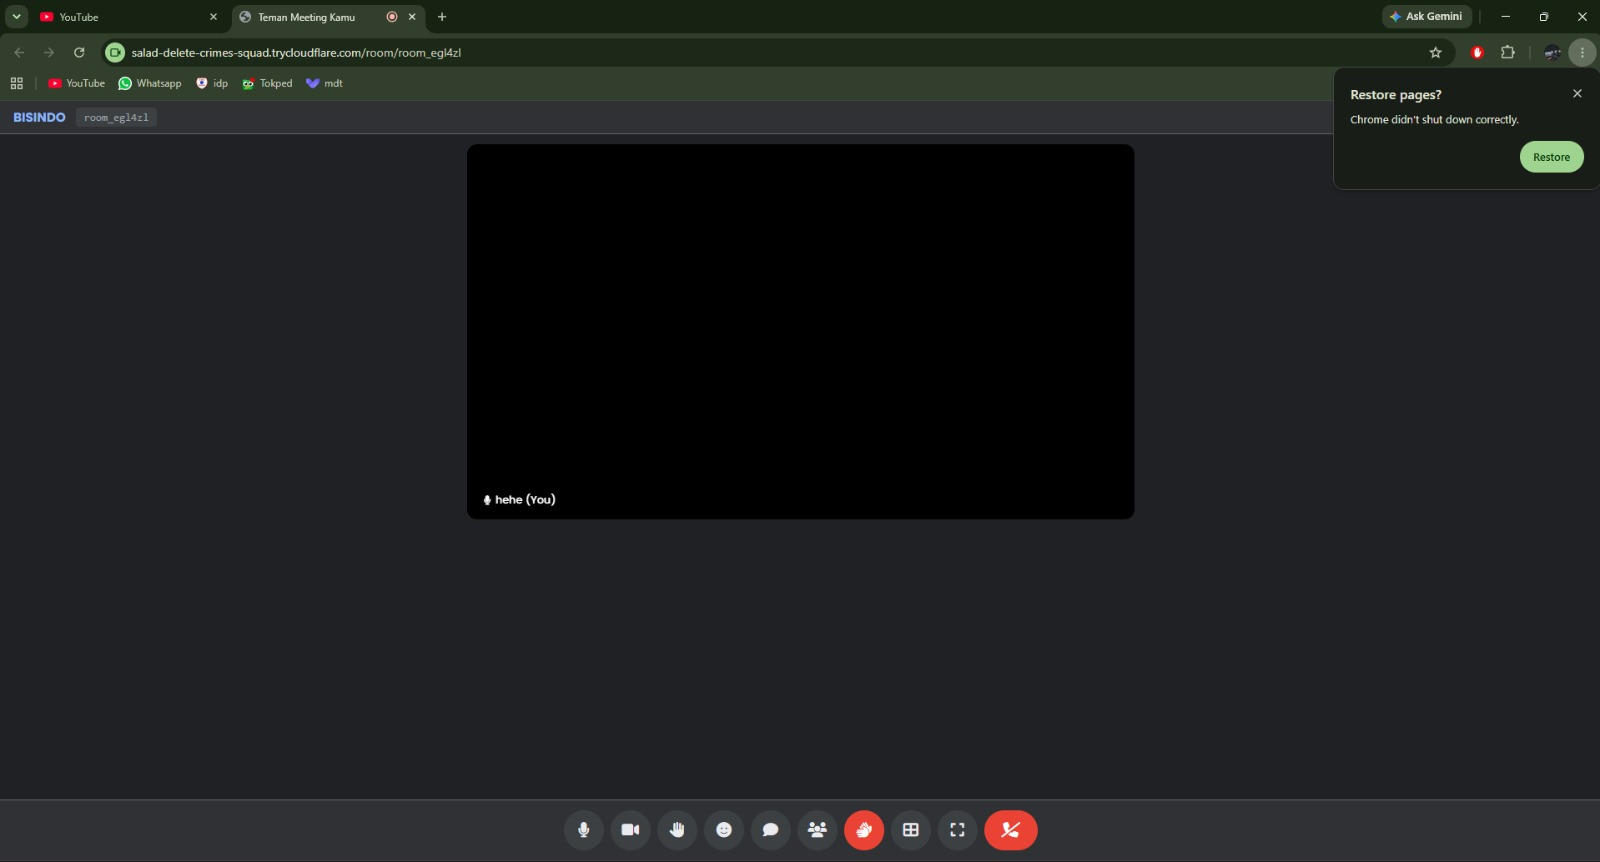
\includegraphics[width=\linewidth]{figures/eval-screenshots/06-failed-join-blank.jpeg}
\caption{Joined room, blank stage.}
\label{fig:mesh-fail}
\end{subfigure}
\caption{Live failure modes in a six-participant session: (a)~baseline;
(b)~six in roster, four rendered; (c)~black/frozen tiles; (d)~blank stage
after join.}
\label{fig:mesh-evidence}
\end{figure}

At $N=2$ the mesh connects reliably, with both peers receiving
audio and video and no drops. Larger rooms degraded clearly. In a live
session peaking at six concurrent participants (of seven to eight
who attempted to join), not all participants could see each other: reception
was asymmetric; some observers rendered four of five remote streams,
others three, at least one peer could not join, and some videos
froze mid-session. These symptoms follow directly from the
$O(n^2)$ full-mesh fan-out, where each peer uploads to every other. The
limiting factor as rooms grow is upstream bandwidth and connection setup,
not recognition, and weaker (mobile/cellular) uplinks fail first, which
motivates the SFU/relay direction in future work.

\textbf{Qualitative evidence.} Figure~\ref{fig:mesh-evidence}
shows the four failure modes live. The roster in
Fig.~\ref{fig:mesh-count} also reveals an unsanitized
SQL-injection-style username stored and rendered verbatim (see
limitations).

\textbf{End-to-end latency and frame rate.} We instrumented the
in-browser pipeline (MediaPipe detection $+$ normalization $+$ ONNX
inference $+$ UI update) with \texttt{performance.now()} over 100
consecutive frames with a hand in view on a laptop with Intel integrated
graphics (Figure~\ref{fig:latency}): \textbf{18.7~FPS mean / 20.4 median}
(15.2 at the P95-worst frame), i.e.\ \textbf{53.4~ms mean / 48.9 median}
(65.7~ms P95). With classifier-only inference at $0.53$~ms, essentially
all per-frame cost is MediaPipe detection and rendering; recognition is
not the bottleneck, and a steady $\approx$20~FPS suffices for the
static-posture alphabet task.
% e2e-fps: measured 2026, Chrome, laptop iGPU, 100 frames via startFpsBench()

\textbf{Broadcast latency.} We timestamped each letter-commit
emit and measured the delay until it rendered on
a remote peer over a live session ($n=190$ committed letters). Because the
clocks were not NTP-synchronized, absolute mean/min values are dominated by
skew and meaningless (the raw mean was negative); we therefore report the
\emph{median}, robust to a constant offset: \textbf{59~ms} median
end-to-end, with a P95 of $\approx$1.6~s from occasional tunnel/network
stalls. The sub-100~ms median shows socket relay to peers is effectively
interactive once a letter is committed; the heavy tail reflects the
best-effort public tunnel, not the recognition or messaging path. A
clock-synchronized re-measurement would tighten the absolute figures.
% broadcast-latency: measured 2026, n=190, median 59ms (mean invalid: clocks unsynced)


% ============================================================
\section{Discussion and Limitations}
\label{sec:limitation}

\textbf{Accuracy vs.\ usability.} The 99.12\% single-hand score is a
useful upper reference under idealized one-hand input, but a communication
tool for BISINDO must accept two hands. The dual-hand model is therefore
the system of record despite a small accuracy gap.

\textbf{Landmarks vs.\ pixels.} Eighty-four floats per frame are enough
for alphabet discrimination while remaining edge-friendly, aligning with
the broader shift toward skeleton-based SLR~\cite{deep-survey}.

\textbf{What the failure modes teach.} The live evaluation is as
informative as the accuracy table. A room can be healthy for one
participant and broken for another on the same network; tiles can go
black or blank while the roster still counts them; and none of this is
visible in an offline metric. The practical consequences are concrete:
keep rooms small, monitor \emph{rendered}-stream counts rather than
roster counts, and treat a media-relaying SFU as the scaling path ---
all of which shape the future work below.

\textbf{Threats to validity.} Three caveats temper the numbers. First,
the 85/15 split is signer-overlapping, so the reported accuracy is
\emph{signer-dependent}; a leave-one-signer-out protocol is the honest
next measurement. Second, all captures share one webcam geometry, one
indoor lighting profile, and a small contributor pool, so accuracy on
unseen rooms, lighting, and skin tones is unmeasured. Third, latency and
frame rate were profiled on a single mid-range laptop CPU; weaker devices
will trade frame rate rather than accuracy, since inference is only
0.53~ms of the 53.4~ms loop.

\textbf{Deployment posture.} Given these bounds we position \kw{BISINDO
Bridge} as a communication aid for familiar partners --- classrooms,
family calls, small team meetings --- where a signer can repeat or
fingerspell after a rare misrecognition, not as an interpreter
replacement. The sentence builder's edit gestures exist precisely because
the human stays in the loop: a fist deletes, a palm clears, and the
conversation continues without breaking the meeting.

\textbf{Limitations.} Table~\ref{tab:limitations} summarizes the eight
limitations that bound deployment claims.

\begin{table}[t]
\caption{Limitations of the current system.}
\label{tab:limitations}
\centering
\setlength{\tabcolsep}{4pt}
\begin{tabular}{@{}p{30mm}p{82mm}@{}}
\toprule
Limitation & Detail \\
\midrule
Data scale \& diversity & $\approx$1{,}000 samples/letter from a small, homogeneous group; strong held-out accuracy but too narrow for production---proof-of-concept, likely to scale with more data. \\
Signer concentration & Few contributors dominate capture; style bias. \\
Capture conditions & Front webcam, indoor, limited viewpoints; M, N, Q mapped to single-handed forms. \\
Evaluation rigor & Single 85/15 split, possible same-signer leakage; 98.45\% likely \emph{signer-dependent}; leave-one-signer-out is the immediate next measurement. \\
Vocabulary scope & 26 alphabet letters with rule-based delimiters, not full lexical BISINDO. \\
Transport \& scale & Full mesh $O(n^2)$, best-effort public TURN (no SFU); quick-tunnel URLs suit demos, not production. \\
UI robustness & Occasional malformed confidence readout (``1017\%''); display-only, classification unaffected. \\
Input hardening & Unsanitized display names (SQL-injection-style string stored verbatim); validation required before production. \\
\bottomrule
\end{tabular}
\end{table}

\section{Conclusion and Future Work}
\label{sec:conclusion}

BISINDO Bridge couples a dual-hand 84-D landmark 1D-CNN (98.45\% Acc/F1,
61{,}274 parameters) with on-device ONNX inference and a full-mesh WebRTC
meeting that broadcasts composed sentences. Every stage of recognition
runs inside the participant's browser, so a video meeting gains
sign-language support without installs, accounts, or server-side vision.

Two results anchor the contribution. On the recognition side, a compact
per-frame classifier is enough for the alphabet when the input is
normalized geometry: three-stage normalization over an 84-D two-hand
representation reaches 98.45\% on held-out samples while consuming
0.53~ms of a 53.4~ms frame budget. On the systems side, the honest
finding is that the media path, not model accuracy, is what limits real
rooms: reception degrades asymmetrically as participants join, which we
document through live failure modes rather than hide.

The design choices that make the tool usable in practice ---
browser-side privacy, ICE-restart recovery, two-hand letter coverage ---
required accepting a small accuracy cost against the single-hand
baseline, and we believe that trade is correct: a communication tool for
BISINDO must accept both hands.

Future work follows directly from the evaluation. For recognition, the
per-frame model is the foundation for \emph{continuous} signing: a
temporal layer over committed letters, a broader vocabulary, and
language modeling can turn the alphabet into flowing phrases. For
evaluation, the immediate next measurement is a leave-one-signer-out
protocol to quantify signer dependence, followed by usability studies
with deaf participants, which this paper deliberately does not claim.
For transport, the full mesh should give way to a media-relaying SFU so
that room size stops being an $O(n^2)$ constraint, with a named tunnel
and input hardening closing the remaining production gaps.

% ============================================================
% NOTE: no \clearpage here (it left a half-empty page); verified no float
% lands after the reference list in the final build.
\begin{thebibliography}{99}

\bibitem{mediapipehands2020}
F.~Zhang, V.~Bazarevsky, A.~Vakunov, A.~Tkachenka, G.~Sung,
C.-L.~Chang, and M.~Grundmann, ``MediaPipe Hands: On-device Real-time
Hand Tracking,'' \textit{arXiv:2006.10214}, 2020.

\bibitem{auziqni2022}
R.~Auziqni, ``BISINDO Indonesian Sign Language Recognition Using MediaPipe
Holistic and LSTM Deep Learning Model,'' Undergraduate thesis, Universitas
Mercu Buana, Jakarta, Indonesia, 2022.
\url{https://repository.mercubuana.ac.id/id/eprint/69873}, accessed 2026.

\bibitem{bisindo-lstm-2023}
T.~M.~A.~Afwan, R.~Gernowo, and H.~A.~Wibawa, ``Deep Learning-Based
Recognition of Indonesian Sign Language (BISINDO) Alphabetic Gestures
Using Skeletal Feature Extraction and LSTM,'' \textit{Jurnal Teknik
Informatika (Jutif)}, vol.~7, no.~2, 2026, doi:
\nolinkurl{10.52436/1.jutif.2026.7.2.5337}.

\bibitem{cnn-lstm-bp}
A.~Aljabar and Suharjito, ``BISINDO (Bahasa Isyarat Indonesia) Sign
Language Recognition Using CNN and LSTM,'' \textit{Advances in Science,
Technology and Engineering Systems Journal}, vol.~5, no.~5,
pp.~282--287, 2020, doi: \nolinkurl{10.25046/aj050535}.

\bibitem{deep-survey}
R.~Rastgoo, K.~Kiani, and S.~Escalera, ``Sign Language Recognition: A Deep
Survey,'' \textit{Expert Systems with Applications}, vol.~164,
Art.~no.~113794, 2021.

\bibitem{deepsign-access}
M.~Al-Qurishi, T.~Khalid, and R.~Souissi, ``Deep Learning for Sign Language
Recognition: Current Techniques, Benchmarks, and Open Issues,''
\textit{IEEE Access}, vol.~9, pp.~126917--126951, 2021.

\bibitem{hand-review}
M.~Oudah, A.~Al-Naji, and J.~Chahl, ``Hand Gesture Recognition Based on
Computer Vision: A Review,'' \textit{Journal of Imaging}, vol.~6, no.~8,
Art.~no.~73, 2020.

\bibitem{bisindo-cnn-mediapipe}
A.~K.~Fadzli and M.~Rahardi, ``Comparative Analysis of MobileNetV3 and
EfficientNetv2B0 in BISINDO Hand Sign Recognition Using MediaPipe
Landmarks,'' \textit{Journal of Applied Informatics and Computing},
vol.~10, no.~1, 2026, doi: \texttt{10.30871/jaic.v10i1.11878}.

\bibitem{mediapipe-framework}
C.~Lugaresi et al., ``MediaPipe: A Framework for Building Perception
Pipelines,'' \textit{arXiv:1906.08172}, 2019.

\bibitem{1d-cnn-healthcare}
N.~Al~Mudawi \textit{et al.}, ``Innovative Healthcare Solutions: Robust
Hand Gesture Recognition of Daily Life Routines Using 1D CNN,''
\textit{Frontiers in Bioengineering and Biotechnology}, vol.~12,
Art.~no.~1401803, 2024, doi: \texttt{10.3389/fbioe.2024.1401803}.

\bibitem{mediapipe-review}
K.~Kumar et al., ``Mediapipe and CNNs for Real-Time ASL Gesture
Recognition,'' \textit{arXiv:2305.05296}, 2023.

\bibitem{onnx}
Microsoft, ``ONNX Runtime,'' documentation,
\url{https://onnxruntime.ai}, accessed 2026.

\end{thebibliography}

\end{document}
